\chapter[Tonian paleomagnetism from South China permits an inclusive Rodinia or Bitter Springs Stage true polar wander, but not both][Xiajiang Group]{Tonian paleomagnetism from South China permits an inclusive Rodinia or Bitter Springs Stage true polar wander, but not both}

\section{Abstract}

The Tonian supercontinent Rodinia is hypothesized to have included almost all Proterozoic continental blocks. Competing models variably place South China at the core or periphery of Rodinia, or separated from it entirely. Tonian paleogeographic models also vary in whether they incorporate proposed large and rapid oscillatory true polar wander associated with the ca. 810--795~Ma Bitter Springs Stage. Here we develop new paleomagnetic data paired with U-Pb chemical abrasion isotope dilution thermal ionization mass spectrometry (CA-ID-TIMS) zircon geochronology from the Tonian Xiajiang Group in South China to establish the craton's position and test the Bitter Springs Stage true polar wander hypothesis. The Xiajiang Group comprises fine-grained siliciclastic rocks with interbedded volcanic ashes and unconformably overlies folds associated with the Jiangnan Orogeny, which united the Yangtze and Cathaysia blocks of South China. A U-Pb CA-ID-TIMS zircon date of 815.73$\pm$0.18~Ma from a tuff near the base of the Xiajiang Group brackets folding associated with the Jiangnan Orogeny to have occurred between ca. 830 and 816~Ma. Paleomagnetic data from stratigraphic units near the dated horizon constrain South China to high latitudes ca. 813~Ma. These data indicate a relatively stable high-latitude position from the time of the ca. 821~Ma Xiaofeng dikes pole to the ca. 805~Ma Madiyi Formation pole. These high-latitude constraints either connect the craton to Rodinia along its periphery, or disconnect it from the (super)continent entirely. The difference in pole position between the pre-Bitter Springs Stage Xiajiang Group pole and the syn-Bitter Springs Stage Madiyi Formation pole is significantly less than that predicted for the Bitter Springs Stage true polar wander hypothesis. If this pole difference is interpreted as true polar wander superimposed upon differential plate motion, it requires South China to have been separate from Rodinia.

\section{Introduction}

Earth's lithosphere moves through two fundamental mechanisms. The more familiar of these mechanisms are tectonic motions --- that is, differential movement between lithospheric plates. The second mechanism is the rotation of the entire silicate Earth in order to maintain rotational equilibrium. On any rotating planetary body, changes in the distribution of mass on (e.g. the melting of ice sheets; \citealp{Mitrovica2005a, Matsuyama2010a, Cambiotti2010a}) or within (e.g. mantle convection; \citealp{Spada1992a}) can cause reorientation of the planetary surface relative to the rotational axis \citep{Evans2003a, Matsuyama2014a}. Such reorientation causes all of Earth's tectonic plates, as well as the underlying mantle, to rotate in unison relative to the spin axis and the core. To an observer on Earth's surface, it would appear that the pole is changing position and the process is therefore referred to as true polar wander (TPW). Differential plate tectonics and TPW are operating today and were in Earth's past. Both processes are built into paleogeographic models over the past 400 million years (m.y.), with an overall dominance of differential plate tectonics \citep{Steinberger2008a, Torsvik2012a}.

Plate kinematic reconstructions indicate that the median plate velocity over the past 200~m.y., during which a seafloor spreading record is preserved, is $\sim$4~cm/yr \citep{Zahirovic2015a}. Although plate velocities have been observed to significantly exceed this median value, such as during the rapid northward motion of India toward Eurasia ca. 55~Ma when its velocity was as high as 19~cm/yr \citep{Hinsbergen2011a, Zahirovic2012a}, such motions are short-lived (up to $\sim$10~m.y.; \citealp{Zahirovic2015a}). Based on these plate kinematic reconstructions, it has been argued that plate velocities rarely exceed $\sim$20~cm/yr \citep{Meert1993a, Zahirovic2015a}.

Over the past 300~m.y., there has been near continuous TPW at rates of 1--10~cm/yr due to advection of mass heterogeneities in the mantle \citep{Steinberger2008a, Torsvik2012a}, with the possibility of more rapid TPW in the Jurassic \citep{Kent2015a}. These rates are comparable to rates of differential plate motion, which can make TPW difficult to distinguish in the record. The possibility of TPW occurring at rates exceeding those of typical plate tectonics has been discussed as a theoretical possibility in the geophysical literature \citep{Gold1955a, Fisher1974a, Steinberger1997a, Evans2003a}, and has been proposed as an explanation for large shifts in paleomagnetic poles in the geological record. The rate at which true polar wander can occur is a function of the magnitude of the perturbation to Earth's moment of inertia tensor, the timescale over which that perturbation is applied, and the timescale for viscoelastic adjustment of Earth's rotational bulge, which is itself largely a function of mantle viscosity \citep{Tsai2007a, Steinberger2010a, Creveling2012a}. Additionally, stabilization is thought to result from TPW-induced stresses in the lithosphere that can form a remanent bulge \citep{Ricard1993a, Chan2014a}. Numerical models have suggested that velocities due to TPW motion can be higher than $\sim$150~cm/yr \citep{Spada1992a}, although other treatments have argued that TPW exceeding $\sim$25~cm/yr is unlikely \citep{Tsai2007a}. Ultimately, however, the rate at which TPW has proceeded at different periods of Earth history is a question for geologic and paleomagnetic records.

A pair of oscillatory TPW events ca. 810 and 795~Ma have been proposed to have occurred during the Tonian Period of the Neoproterozoic Era \citep{Maloof2006a}. This hypothesis is based on paleomagnetic, isotopic, and stratigraphic data from carbonate strata in the Akademikerbreen Group of East Svalbard --- a terrane that was part of Laurentia in the Tonian \citep{Maloof2006a}. Two \textgreater50\degrees shifts in paleomagnetic direction from Svalbard, with associated plate velocities interpreted to be \textgreater50~cm/yr, were observed to be coincident with abrupt shifts in \dC (referred to as the Bitter Springs Stage; \citealp{Maloof2006a}). Furthermore, these different poles were from different carbonate facies and are separated by unconformities that were interpreted to reflect the transient changes in local relative sea level predicted to occur given the differential response of the fluid and solid Earth \citep{Mound1999a, Maloof2006a}. These shifts were interpreted as `there and back again' TPW rotations in which the entire solid Earth (and therefore all of Rodinia) rotated 50\degrees about an equatorial axis and then returned to near its prior position \citep{Maloof2006a}. Further geochronologic constraints on \dC records correlated to the Bitter Springs Stage, and therefore the proposed oscillatory TPW, constrain it to have started after 811.51$\pm$0.25~Ma (U-Pb CA-ID-TIMS zircon from a tuff $\sim$50~m below carbonates that record the first abrupt shift to negative \dC values in the Fifteenmile Group of northwest Canada; \citealp{Macdonald2010a}) and to have ended by 788.72$\pm$0.24~Ma (U-Pb CA-ID-TIMS zircon from a tuff $\sim$250~m above carbonates that record the second abrupt shift to positive \dC values in the Tambien Group of northern Ethiopia; \citealp{Swanson-Hysell2015a, Park2020a}). Interpolation using these and other geochronologic constraints suggest that the Bitter Springs Stage started before 807.9$\pm$0.2~Ma and ended after 800.6$\pm$0.2~Ma \citep{Swanson-Hysell2015a}. However, no direct geochronologic constraints exist on the Akademikerbreen Group stratigraphy, and therefore the ages of these paleomagnetic poles for Svalbard are reliant on carbon and strontium isotope chemostratigraphic correlations \citep{Halverson2007a}.

Given that TPW results in rotation of the entire lithosphere around the spin axis, it should manifest in the paleomagnetic record as simultaneous and identical motion of paleomagnetic poles across all continents, once standard differential plate tectonic motion has been subtracted out \citep{Evans2003a}. Efforts to test the Bitter Springs Stage TPW hypothesis within the Bitter Springs Group of central Australia led to distinct paleomagnetic pole positions from syn-Bitter Springs Stage and post-Bitter Springs Stage sedimentary rocks \citep{Swanson-Hysell2012a}. The post-Bitter Springs Stage pole was developed from a hematite remanence held in Johnny's Creek Formation siltstone and is included as a constraint for Australia in models of Rodinia (e.g. \citealp{Merdith2017a}). The syn-Bitter Springs Stage pole from Love's Creek Formation carbonate overlaps with the Cambrian apparent polar wander path of Australia, raising the possibility that the difference in position between the Love's Creek and Johnny's Creek poles is the result of remagnetization, leaving ambiguity in using these data to test the TPW hypothesis \citep{Swanson-Hysell2012a}. The paleomagnetic remanence of carbonate rocks can be challenging to interpret as they are prone to remagnetization \citep{Van-Der-Voo2012a, Jackson2012a}. Carbonate remagnetization can be particularly vexing as it can result from chemical alteration at low temperatures such as the conversion of smectite to illite. This process can lead to the authigenic formation of magnetite at temperatures as low as 70\degreesC \citep{Katz1998a, Tohver2008a}. This mechanism may explain the magnetization obtained from carbonates of the Love's Creek Formation of the Bitter Springs Group as a Cambrian overprint from authigenic magnetite formation during burial \citep{Swanson-Hysell2012a}. These potential complexities highlight the importance of testing the Bitter Springs TPW hypothesis using other lithologies such as detrital hematite-bearing siliciclastics and igneous rocks.

Tonian deposition in the Nanhua Basin of South China includes reds beds and volcanic tuffs. These units potentially span the Bitter Spring Stage and provide an opportunity to develop high quality paleomagnetic data paired with precise geochronology to test both the Bitter Springs TPW hypothesis and models of the configuration of the Neoproterozoic supercontinent Rodinia.

\section{Paleogeographic Setting}

\begin{figure}[h!]
    \centering
    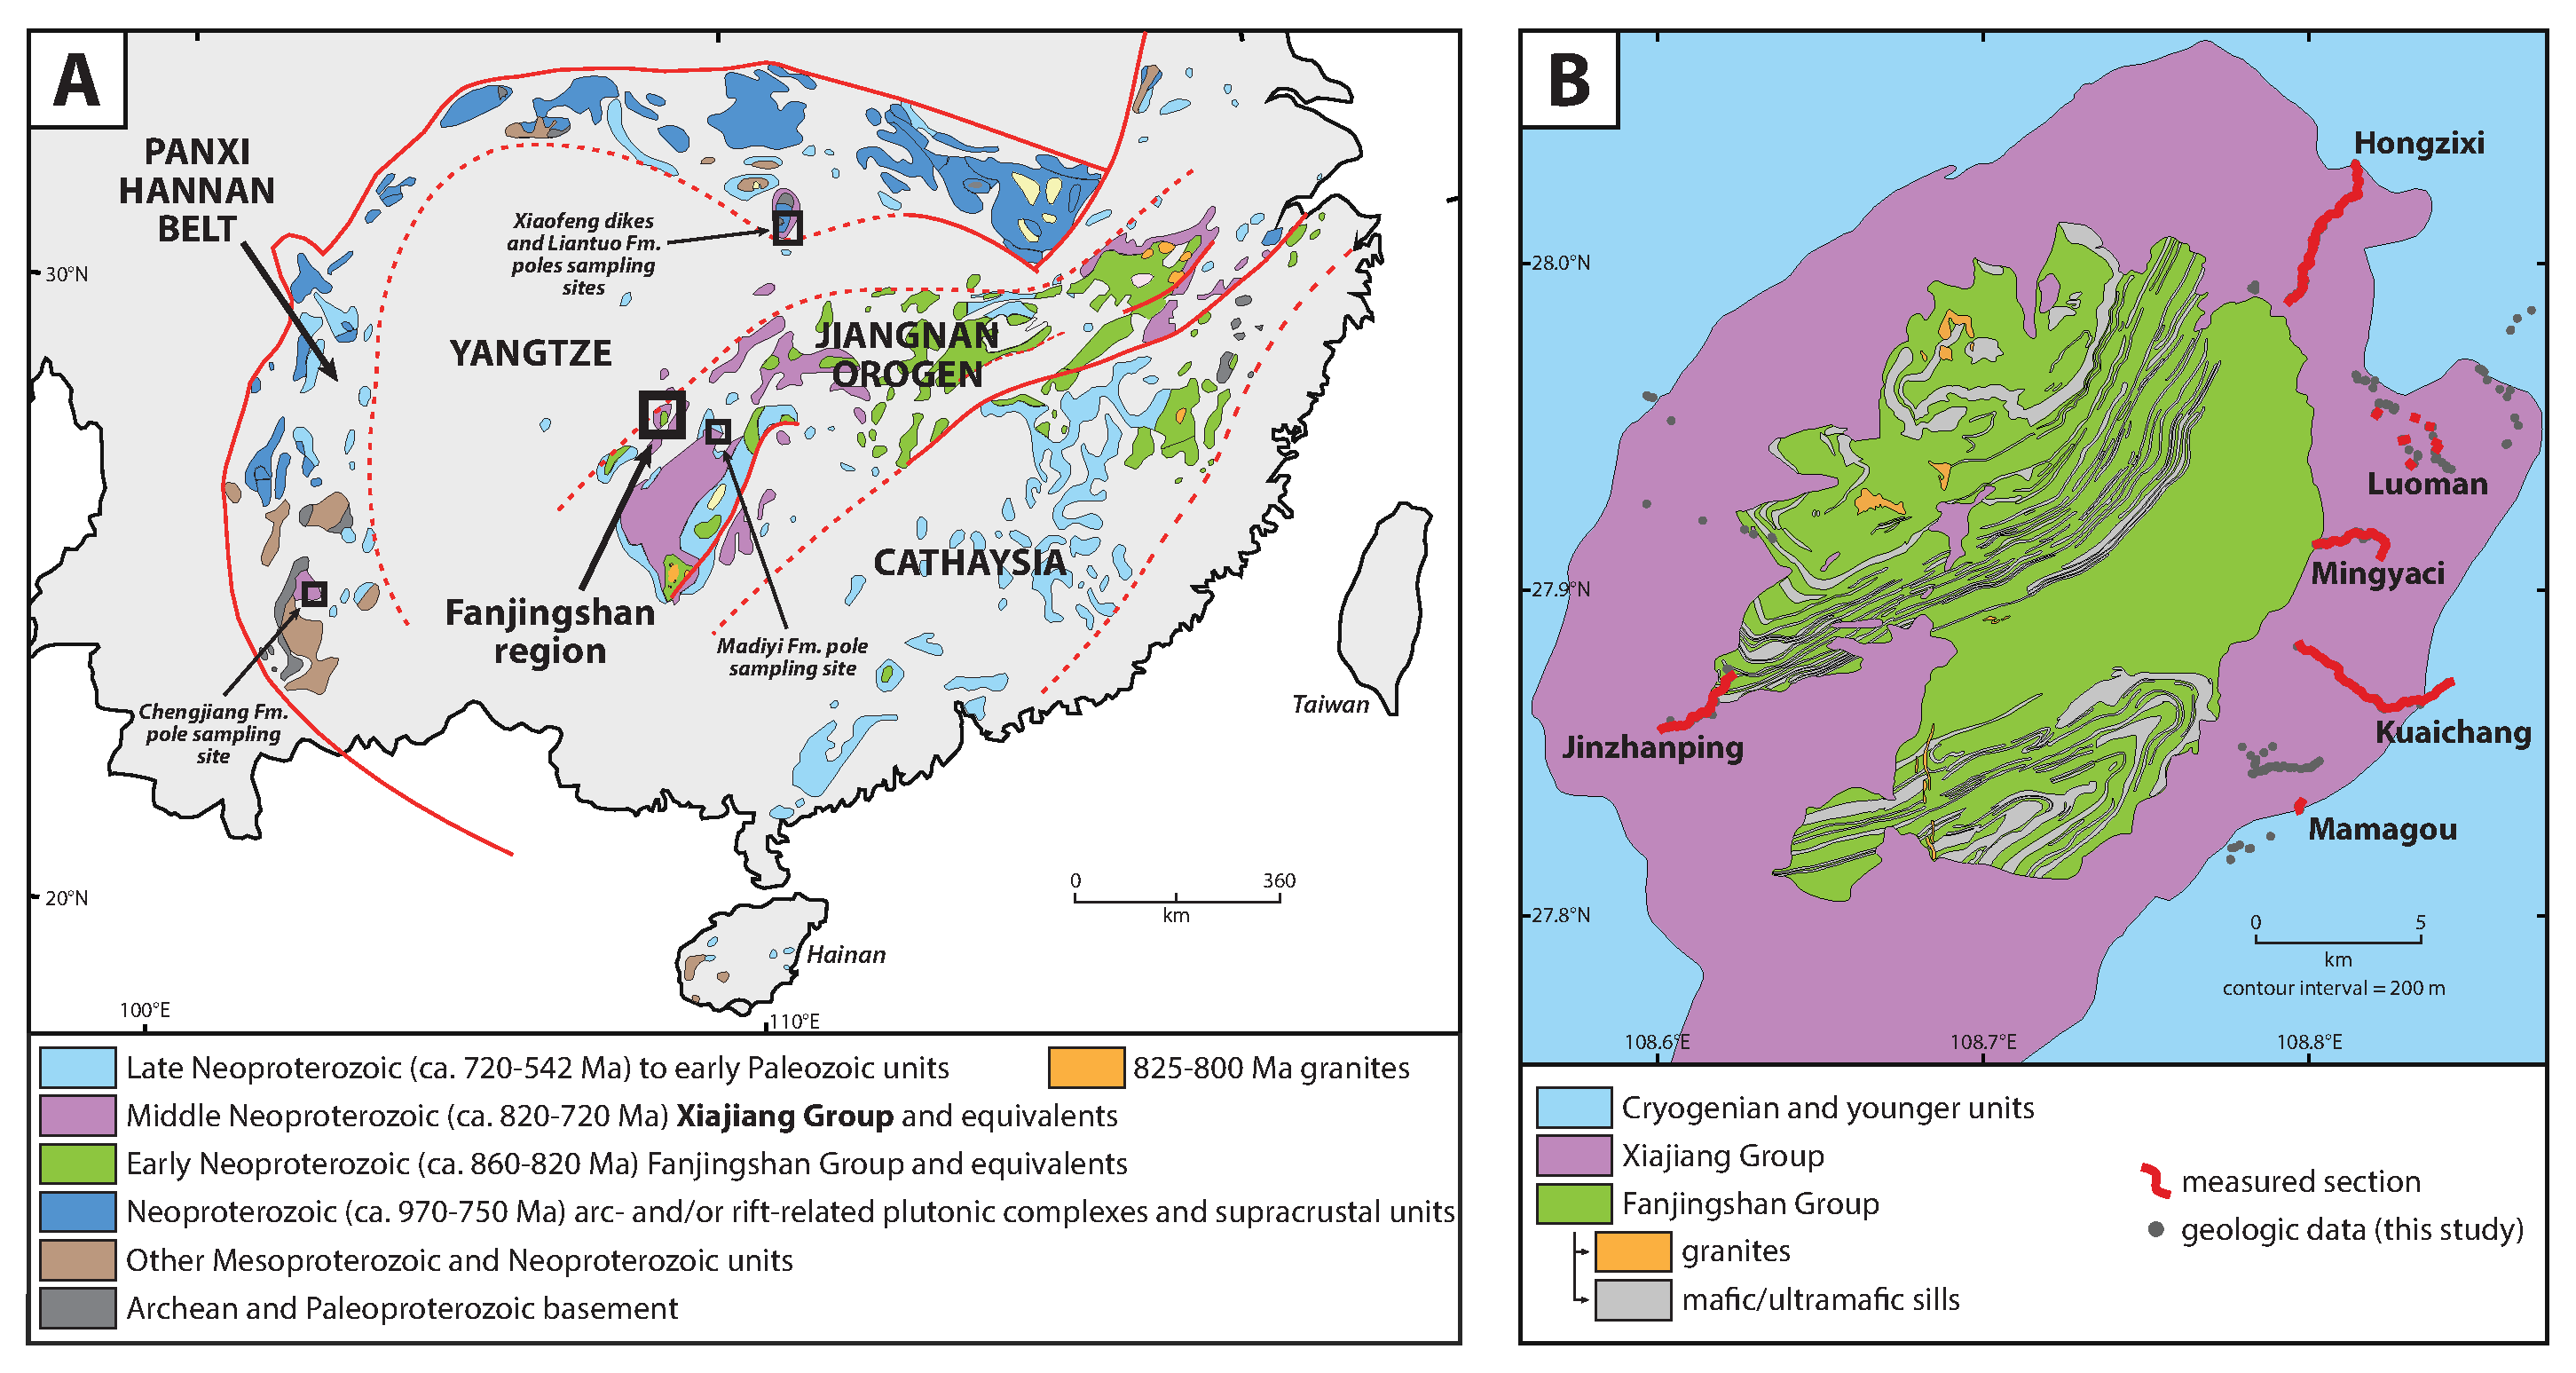
\includegraphics[width=1\textwidth]{figures/Xiajiang/geologic-maps.pdf}
    \caption[Geologic maps of South China and the Fanjingshan region.]{\textbf{A)} Summary geologic map of South China, adapted from \citet{Cawood2017a}, showing the Fanjingshan region from where the Xiajiang Group pole is developed in this study, as well as the localities where other Neoproterozoic poles are developed (Table \ref{tab:South-China-poles}). \textbf{B)} Geologic map of the Fanjingshan region. The distribution of volcanic units within the Fanjingshan Group and the contact between the Fanjingshan and Xiajiang groups were adapted from \citet{Wang2016c}. Both the sedimentary and volcanic units of the Fanjingshan Group were folded, uplifted, and eroded prior to Xiajiang Group deposition. The contact between the Xiajiang Group and the overlying Cryogenian units was adapted from \citet{Zhao2011a}. Unit boundaries were adjusted to be consistent with our geologic data where available. Red lines show the location of the measured stratigraphic sections in Figure \ref{fig:stratigraphic-sections}. Note that the Luoman section consists of seven individually measured sections that were correlated to each other based on local bedding and elevation measurements.}
    \label{fig:geologic-maps}
\end{figure}

\begin{figure}[h!]
    \centering
    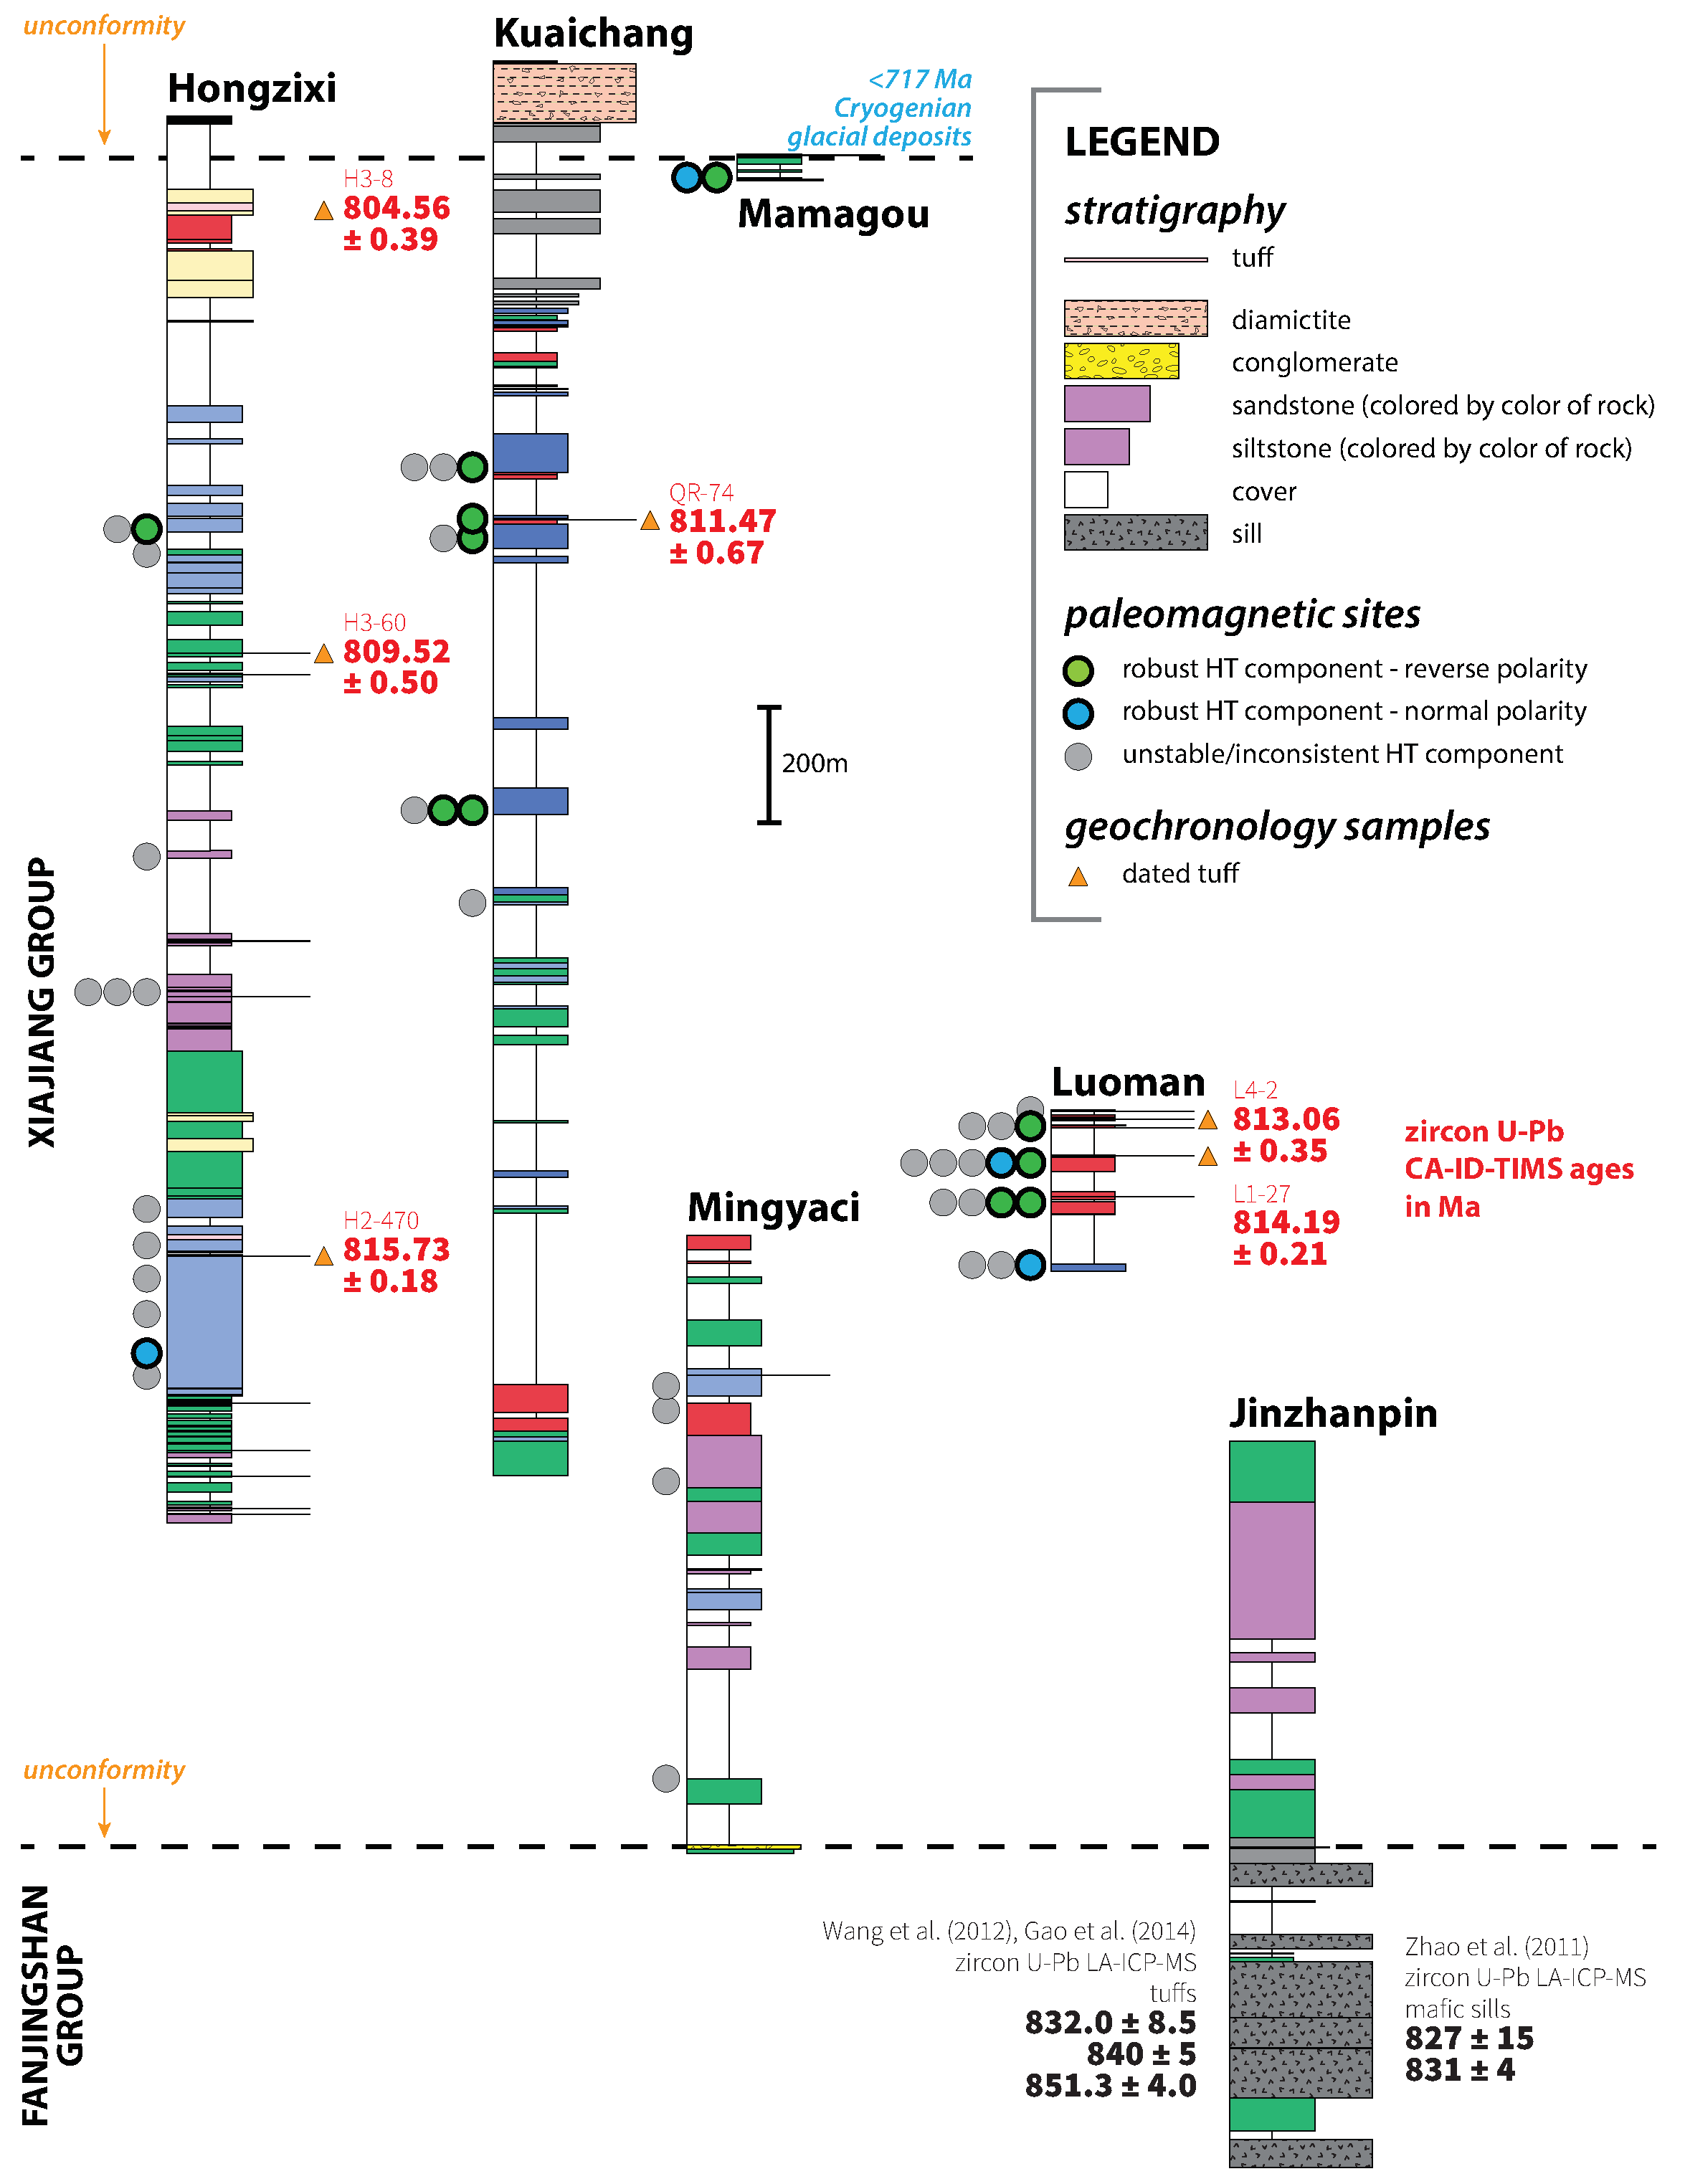
\includegraphics[width=0.80\textwidth]{figures/Xiajiang/stratigraphic-sections.pdf}
    \caption[Stratigraphic sections measured in the Fanjingshan region.]{Stratigraphic sections measured in the Fanjingshan region. Locations of measured sections are shown in Figure \ref{fig:geologic-maps}. The colors are associated with the color of the sedimentary rocks. U-Pb CA-ID-TIMS dates from the Xiajiang Group are from this study and are shown at the stratigraphic levels where the tuffs were collected. The dates from the Fanjingshan Group are not from the section shown, but are from other studies of the rocks elsewhere in the region.}
    \label{fig:stratigraphic-sections}
\end{figure}

Many Proterozoic continental blocks are hypothesized to have come together to form the supercontinent Rodinia during the latest Mesoproterozoic to Neoproterozoic \citep{Hoffman1991a, Li2008a}. However, geochronologic, geologic, and paleomagnetic research continues to refine the configuration of these blocks as well as the timing of their assembly and breakup. At the center of debates regarding the configuration of Rodinia is the South China craton (Fig. \ref{fig:geologic-maps}). For many years, the most widely-used paleogeographic models for the Neoproterozoic adopted the Missing Link model \citep{Li1995a, Li2008a}, which places South China at the core of Rodinia between Australia-East Antarctica and Laurentia. This hypothesis was originally based on the interpretation that the Jiangnan Orogen between the Yangtze and Cathaysia blocks that comprise the South China craton was of similar age to the Grenvillian Orogen of Laurentia (ca. 1.1-1.0~Ga; \citealp{Li1995a}). In this model, the Yangtze block (along with Australia) collides with the Cathaysia block and Laurentia ca. 1.0~Ga \citep{Li1995a}.

Recent geologic, geochemical, and geochronological data have instead interpreted the Jiangnan Orogen to record ongoing accretionary orogenesis of magmatic arc and back arc assemblages along the southeast margin of the Yangtze block in the Tonian up until \textless830~Ma terminal collision with Cathaysia \citep{Cawood2017a, Yan2019a}. In addition to this record of later Tonian magmatism and orogenesis between the Yangtze and Cathaysia blocks, there was accretionary orogenesis and continental arc volcanism along the Panxi-Hannan Belt of the northwest Yangtze block \citep{Cawood2017a}. This record includes both the obduction of ca. 800~Ma ophiolites \citep{Zhao2017a} and ca. 870-706~Ma arc-related magmatism \citep{Dong2012a}. These data indicate that South China was surrounded by active margins with subduction zones through much of the Tonian. This record is difficult to reconcile with a position in the interior of a stable supercontinent. Instead, these data suggest that South China was on the periphery of Rodinia \citep{Cawood2017a}, or disconnected from it entirely \citep{Merdith2017a}. Nevertheless, the Missing Link position for South China, as implemented in \citet{Li2008a}, remains the default in many depictions of Neoproterozoic paleogeography.

\section{Geologic Setting}

This study presents paleomagnetic and U-Pb chemical abrasion isotope dilution thermal ionization mass spectrometry (CA-ID-TIMS) zircon geochronologic data from the Xiajiang Group in the Fanjingshan region of Guizhou province, China (Fig. \ref{fig:geologic-maps}A). The Fanjingshan region lies within the Jiangnan orogenic belt that separates the Yangtze and Cathaysia blocks of the South China craton, and is characterized by a regional anticline that developed in the Mesozoic (Fig. \ref{fig:geologic-maps}B; \citealp{Li2016c, Ma2019a}). At the core of the anticline is the Fanjingshan Group, dominantly composed of sandstones intruded by intermediate to ultramafic sills (Fig. \ref{fig:geologic-maps}B; \citealp{Wang2014a}). These sills are interpreted to have formed in a subduction-related environment just prior to amalgamation of the Yangtze and Cathaysia blocks \citep{Wang2014a}.

Both the sedimentary rocks and the intrusive sills of the Fanjingshan Group are folded, and are separated from the overlying Xiajiang Group by an angular unconformity (Fig. \ref{fig:geologic-maps}B). Tuffs of the Fanjingshan Group in the Fanjingshan region have yielded U-Pb laser ablation inductively coupled plasma mass spectrometry (LA-ICP-MS) zircon dates of 851.3$\pm$4.0~Ma, 840$\pm$5~Ma, and 832.0$\pm$8.5~Ma \citep{Wang2012d, Gao2014a}. U-Pb LA-ICP-MS zircon dates for the mafic sills are 831$\pm$4~Ma and 827$\pm$15~Ma \citep{Zhao2011a}, and U-Pb LA-ICP-MS detrital zircon dates within the sediments are as young as 849$\pm$6.5~Ma \citep{Zhao2011a}. These dates constrain the exposure, folding, and erosion of the Fanjingshan Group to have been after ca. 830~Ma. A cobble to boulder conglomerate is often the lowest unit of the Xiajiang Group, before the stratigraphy transitions into hundreds of meters of red, purple, green, and grey-blue graded beds of siltstone and fine-grained sandstone interbedded with volcanic ashes (Fig. \ref{fig:stratigraphic-sections}). The fine-grained sandstone-siltstone interbeds locally exhibit ripple cross-stratification, which are interpreted to have formed as Bouma-C beds associated with distal turbidity currents. The presence of $\sim$1--5~cm volcanic ashes throughout the stratigraphy without lithic fragments indicate the presence of a nearby, but not immediately adjacent, volcanic arc. Existing U-Pb LA-ICP-MS zircon dates for tuffs of the Xiajiang Group in the Fanjingshan region of 814.0$\pm$6.3~Ma and 813.5$\pm$9.6~Ma \citep{Gao2010a, Gao2014a} suggest deposition of Xiajiang Group began by ca. 815~Ma. Unconformably overlying the Xiajiang Group in the Fanjingshan region are glacial deposits correlated with the Cryogenian Sturtian `Snowball Earth' glaciation (referred to locally as the Chang'an Formation; \citealp{Zhang2011a}). Geochronologic constraints from South China, Laurentia, Oman, and the Arabian-Nubian Shield indicate that onset of the Sturtian glaciation was rapid and globally synchronous within the available precision of the geochronology \citep{Bowring2007a, Macdonald2010a, MacLennan2018a, Lan2020a}. These constraints on the Sturtian glaciation constrain Xiajiang Group deposition to have ended prior to ca. 717~Ma. No continuous individual section was identified that captures both the Fanjingshan-Xiajiang Group contact and the contact between the Xiajiang Group and the Sturtian glacial deposits (Fig. \ref{fig:stratigraphic-sections}). However, correlation of individually measured sections based on aligning the bounding unconformities of the Xiajiang Group and the geochronologic results suggests that the Xiajiang Group is $\sim$3000~m thick in this region (Fig. \ref{fig:stratigraphic-sections}).

We note that the nomenclature of pre-Sturtian Neoproterozoic strata in South China varies in the literature. In some publications, the term the `Banxi Group' is used to refer to any ca. 815--717~Ma sediments in South China, including those in our study area (e.g. \citealp{Zhao2011a, Zhang2019c}). In other publications, the term the `Banxi Group' is used to refer exclusively to ca. 815--717~Ma sediments in the Hunan province, and equivalent strata in our study area in the Guizhou province is referred to as the `Xiajiang Group' (e.g. \citealp{BGMRGZ1984a, Wang2014a, Xiong2014a, Geng2015a, Li2016b, Wang2016c, Yan2019a}). Further to the southeast, sedimentary rocks interpreted to correlate with the Banxi and Xiajiang Groups are referred to as the `Danzhou Group' \citep{Yan2019a}. There are similar regional nomenclature differences for the older Fanjingshan Group, which is referred to as the `Fanjingshan Group' in our study area and is correlated with units known as the `Lengjiaxi Group' and the `Sibao Group' elsewhere. In this study, we follow the nomenclature most widely used for the Guizhou province, using the term Fanjingshan Group, and referring to the sediments unconformably bounded by the Fanjingshan Group and Sturtian glacial deposits in the Fanjingshan region as the Xiajiang Group.

\section{Methods}

\subsection{Paleomagnetism}

Where exposure of the stratigraphy was good, sections were measured using a Jacob’s staff. In cases where vegetation obscured the stratigraphy for hundreds of meters, the thickness of covered stratigraphy was estimated based on GPS measurements and local bedding orientations, leading to the covered intervals shown in Figure \ref{fig:stratigraphic-sections}.

Cores from the studied sedimentary rocks were collected using a gas-powered drill and a Pomeroy orienting device. Sun compass data were used for sample orientations when possible, and magnetic compass orientations were used when necessitated by cloud cover. Sample collection was organized into `sites,' where each site consists of a set of samples that were obtained from within a few meters of stratigraphy. This grouping provides a useful organizational framework although it does not correspond to the definition of a site within the framework of the MagIC database wherein every sample in a site should be expected to record a direction from the same moment in time. In most cases, cores were collected from the least foliated purple/red siltstone of the Xiajiang Group, but when no such lithologies were present, green/grey-blue siltstones were also collected.

Thermal demagnetization and magnetic remanence measurements were conducted at UC Berkeley and the Chinese University of Geosciences. At the UC Berkeley Paleomagnetism Laboratory, measurements were made using a 2G Enterprises DC-SQUID superconducting rock magnetometer equipped with an automated pick-and-place sample changer system \citep{Kirschvink2008a}. The magnetometer is housed in a magnetostatic shield with magnetic fields \textless500~nT. A quartz glass sample rod brings the samples into the measurement region and is typically measured at $\sim5\times10^{-12}$~Am$^{2}$. After measurement of the natural remanent magnetization (NRM), the samples were progressively step-heated and thermally demagnetized in an ASC thermal specimen demagnetizer (residual fields \textless10~nT).

At the Chinese University of Geosciences, paleomagnetic analyses were conducted in a magnetically shielded room with a residual field of \textless300~nT in the Palaeomagnetism and Environmental Magnetism Laboratory. Magnetic remanence was measured using a 2G 755-4~K three-axis cryogenic magnetometer, and stepwise thermal demagnetizations were carried out with an ASC TD-48 or MMTDSC furnace, both of which have an internal residual field of \textless10~nT.

All paleomagnetic data to the measurements level, as well as interpreted fits made using the PmagPy software package \citep{Tauxe2016a}, are available in the MagIC database (https://earthref.org/MagIC/doi/).

\subsection{Geochronology}

Tuffs collected for U-Pb geochronology typically appear as $\sim$1--5~cm horizons within the Xiajiang Group of the Fanjingshan region. Their tan/white color is distinguishable from the purple/red/green/grey-blue of the adjacent siltstone and fine sandstone. In some cases, the exposed surface of the tuffs have weathered into a clay-rich unlithified mud, likely due to the weathering of the volcanic ash to clays (e.g. bentonite). In these cases, the mud was removed before sampling of the lithified tuff. All samples were scrubbed with steel brushes to remove any recent detritus prior to further analysis.

Zircon grains were isolated from the bulk rock by standard mineral separation techniques. All zircon grains analyzed in this study employed the protocols and data reduction outlined in \citet{Meyers2012a}. Prior to dissolution, zircon grains were subjected to a modified chemical abrasion in order to remove radiation-damaged zones of the zircon and minimize the effects of Pb loss \citep{Mattinson2005a}. The accuracy of the $^{238}$U/$^{206}$Pb dates presented herein is controlled by the gravimetric calibration of the EARTHTIME U-Pb tracer employed in this study and the determination of the $^{238}$U decay constant \citep{Jaffey1971a, Condon2015a}. Unless stated otherwise, uncertainties on U-Pb dates reported in this manuscript are the internal (analytical) uncertainties in the absence of external or systematic errors, with these additional uncertainties reported in Table \ref{tab:SChina-geochronology}.

\section{Results}

\subsection{Paleomagnetism}

\begin{table}[h!]
\caption[Paleomagnetic results for the Xiajiang Group of the Fanjingshan region.]{Paleomagnetic results for individual sites with stable and consistent high temperature components in the Xiajiang Group of the Fanjingshan region.}
\vspace{0.25cm}
\resizebox{\linewidth}{!}{
	\begin{tabular}{lllccccccccc}
	\hline
	\textbf{site} & \textbf{section} & \textbf{lab} & \textbf{site lat.} & \textbf{site lon.} & \textbf{n} & \textbf{dec$_{1.0}$} & \textbf{inc$_{1.0}$} & \textbf{dec$_{0.6}$} & \textbf{inc$_{0.6}$} & \textbf{$\alpha_{95}$} & \textbf{polarity} \\
	&&&&&&&&&&& \\
    TR007 & Hongzixi & Beijing & 27.991 & 108.797 & 13 & 14.1 & 64.4 & 14.1 & 73.9 & 8.9 & N \\
    TR014 & Hongzixi & Berkeley & 28.014 & 108.805 & 12 & 150.2 & -66.8 & 330.2 & 75.6 & 12.1 & R \\
    TR018 & Kuaichang & Berkeley & 27.867 & 108.820 & 14 & 208.3 & -64.0 & 28.3 & 73.7 & 14.2 & R \\
    TR020 & Kuaichang & Berkeley & 27.866 & 108.821 & 10 & 111.6 & -76.9 & 291.6 & 82.1 & 11.2 & R \\
    TR021 & Kuaichang & Beijing & 27.864 & 108.822 & 9 & 208.0 & -71.5 & 28.0 & 78.6 & 17.0 & R \\
    TR024 & Kuaichang & Berkeley & 27.872 & 108.811 & 9 & 124.9 & -63.5 & 304.9 & 73.3 & 18.2 & R \\
    TR026 & Kuaichang & Berkeley & 27.872 & 108.811 & 9 & 150.3 & -85.7 & 330.3 & 87.4 & 16.0 & R \\
    TR004a & Mamagou & Berkeley & 27.835 & 108.797 & 10 & 334.8 & 71.4 & 334.8 & 78.6 & 8.2 & N \\
    TR004b & Mamagou & Berkeley & 27.835 & 108.797 & 5 & 106.4 & -75.9 & 286.4 & 81.4 & 12.6 & R \\
    TR031 & Luoman & Beijing & 27.938 & 108.831 & 8 & 337.6 & 65.2 & 337.6 & 74.5 & 14.5 & N \\
    TR034 & Luoman & Beijing & 27.939 & 108.831 & 11 & 291.6 & -75.9 & 111.6 & 81.5 & 13.0 & R \\
    TR035 & Luoman & Berkeley & 27.954 & 108.821 & 19 & 42.4 & 68.4 & 42.4 & 76.6 & 14.9 & N \\
    TR037 & Luoman & Beijing & 27.946 & 108.829 & 17 & 202.1 & -86.3 & 22.1 & 87.8 & 17.2 & R \\
    TR039 & Luoman & Beijing & 27.946 & 108.829 & 9 & 136.8 & -78.1 & 316.8 & 82.8 & 21.2 & R \\
    TR042 & Luoman & Berkeley & 27.943 & 108.839 & 14 & 131.5 & -71.9 & 311.5 & 78.9 & 11.5 & R \\
	\hline
	\end{tabular}}

\scriptsize
\flushleft \emph{Notes:} \\
(1) All directions are for the high temperature component.\\
(2) \textbf{dec$_{1.0}$} and \textbf{inc$_{1.0}$} refer to the declination and inclination of the mean tilt-corrected direction, without correcting for polarity or inclination shallowing.\\
(3) \textbf{dec$_{0.6}$} and \textbf{inc$_{0.6}$} refer to the declination and inclination of the mean tilt-corrected direction, after correcting for polarity and inclination shallowing using a flattening factor of 0.6.\\
(4) For the \textbf{polarity}, N refers to normal polarity in which the inclination of the mean direction is positive, and R refers to reversed polarity in which the inclination of the mean direction is negative.
\label{tab:site-means}
\end{table}

\begin{figure}[h!]
    \centering
    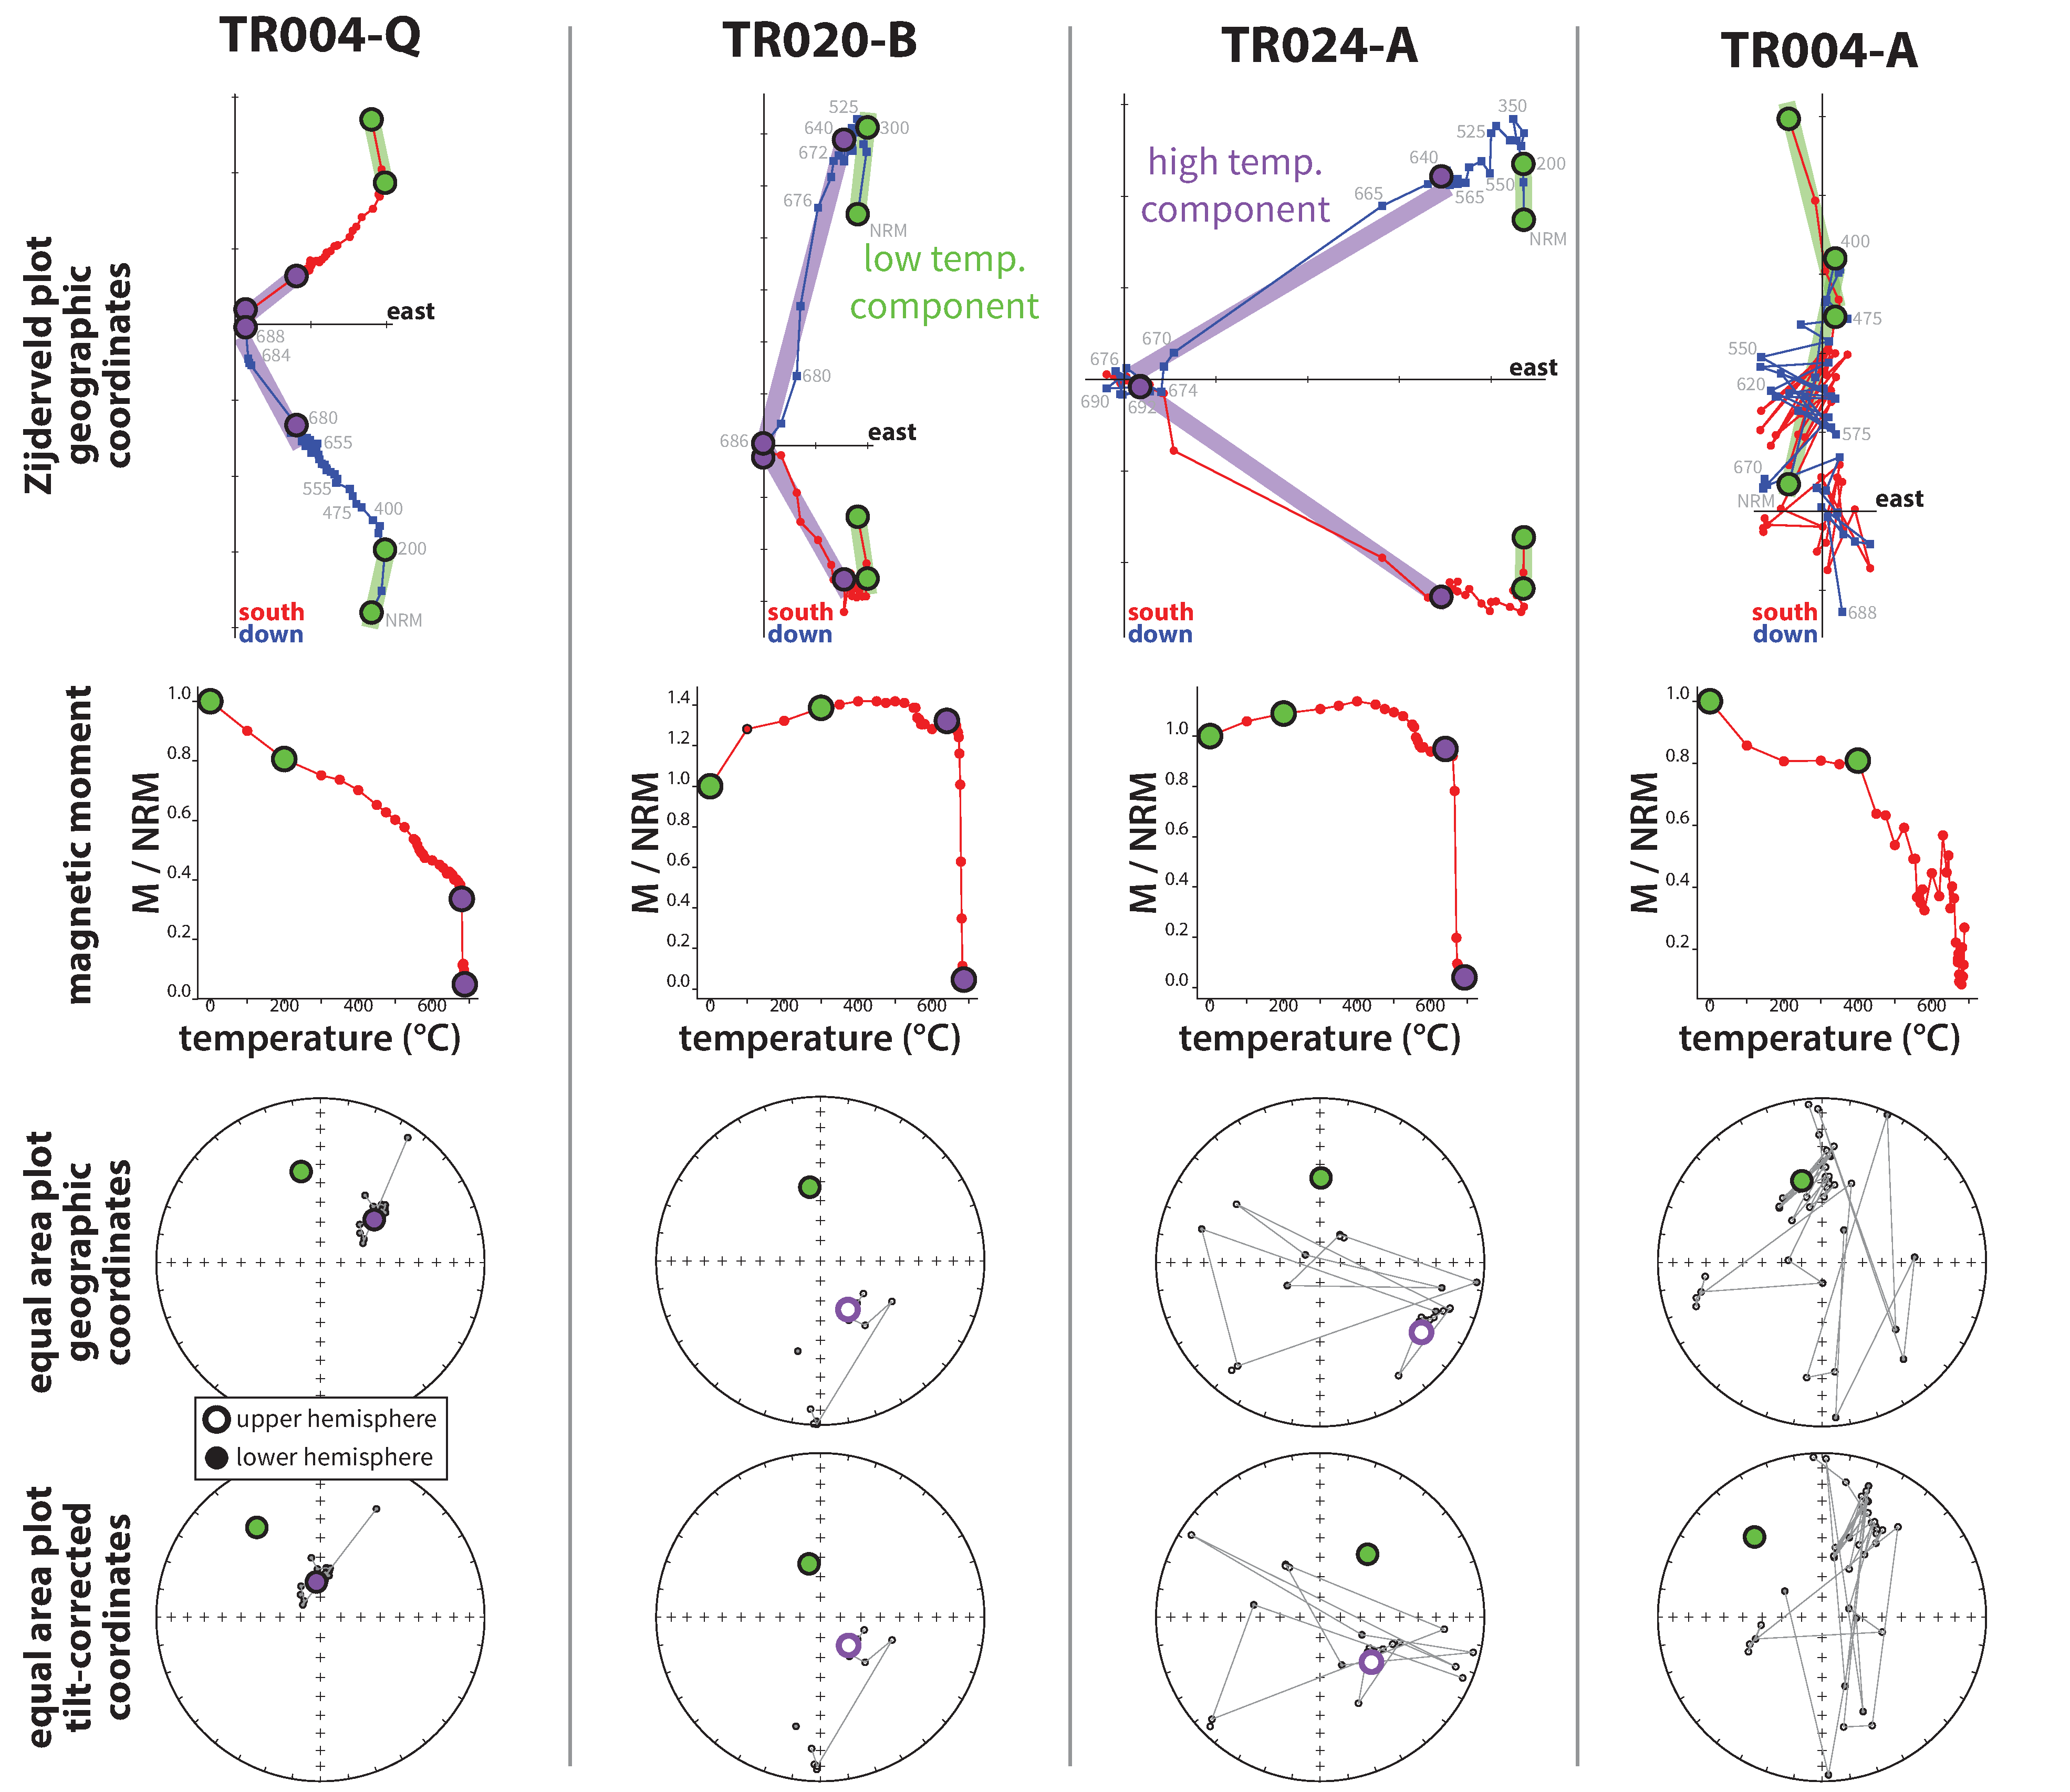
\includegraphics[width=\textwidth]{figures/Xiajiang/representative-specimens.pdf}
    \caption[Thermal demagnetization results.]{Thermal demagnetization results. Specimens TR004-Q, TR020-B, and TR024-A exhibit magnetic behaviour typical of specimens that yield a stable and consistent high temperature component. Specimen TR004-Q exhibits magnetic behaviour typical of specimens that do not yield a stable high temperature component. In the Zijderveld plots, the specimen magnetizations at a given thermal demagnetization step (grey numbers) are shown (NRM = natural remanent magnetization). Fits to the low and high temperature components are shown in green and purple respectively. Note that the Zijderveld plots and the upper equal area plots are in geographic coordinates, whereas the lower equal area plot is in tilt-corrected coordinates.}
    \label{fig:representative-specimens}
\end{figure}

\begin{figure}[h!]
    \centering
    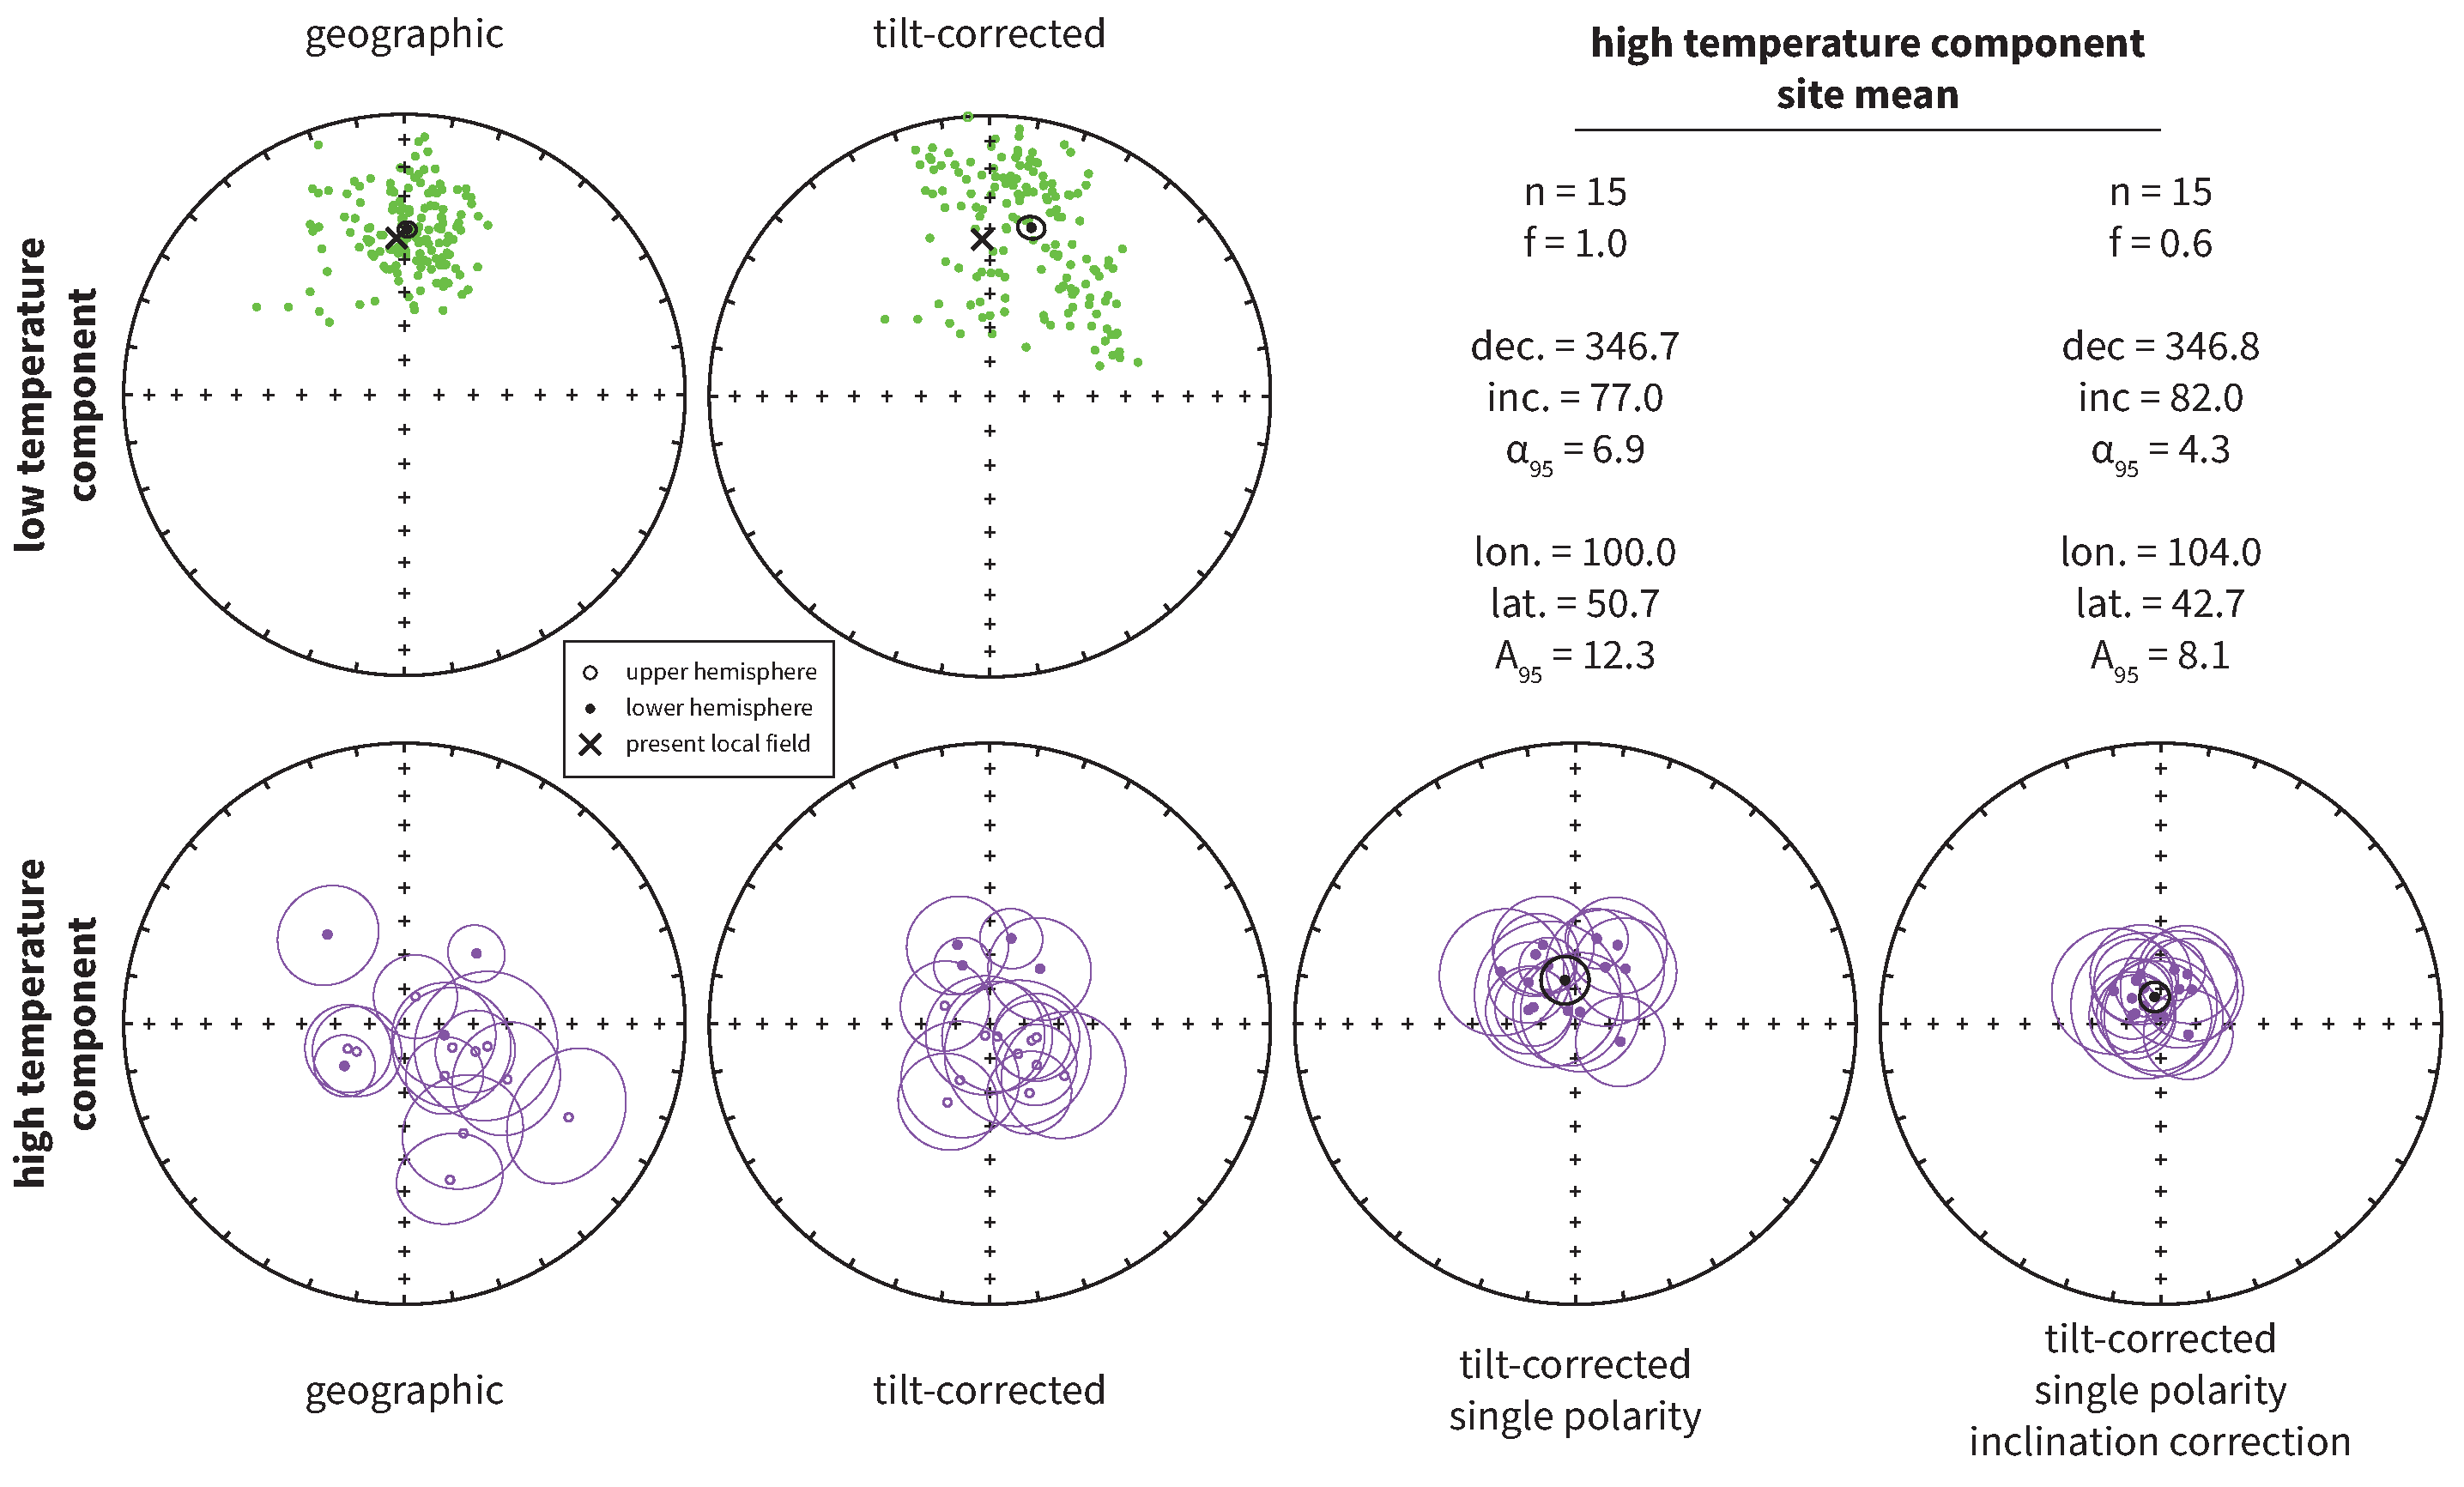
\includegraphics[width=\textwidth]{figures/Xiajiang/site-means.pdf}
    \caption[Paleomagnetic results for the Xiajiang Group of the Fanjingshan region.]{Paleomagnetic results for sites that yielded specimens with stable and consistent high temperature components in the Xiajiang Group of the Fanjingshan region (Table \ref{tab:site-means}). For the low temperature component, each point represents an individual specimen. For the high temperature component, each point and associated uncertainty ellipse represents the specimen mean for individual sites. The reported site means are the means of these specimen means.}
    \label{fig:site-means}
\end{figure}

Thermal demagnetization data from siltstones of the Xiajiang Group in the Fanjingshan region show variable behaviour from site to site. A component removed during initial thermal demagnetization steps (\textless300\degreesC) is present in most samples and typically yields a direction that is consistent with a present local field overprint acquired via viscous remanent magnetization (Fig. \ref{fig:representative-specimens}). Samples within 29 of the 44 sites yield either unstable or inconsistent behaviour at temperatures \textgreater300\degreesC. However, the remaining 15 sites yield stable and consistent behaviour at high temperatures. This high-temperature component is well-fit by least-squares lines that intersect the origin on a Zijderveld plot between $\sim$650 and $\sim$690\degreesC (Fig. \ref{fig:representative-specimens}). These high unblocking temperatures are close to the N\'eel temperature of \textgreater500~nm hematite, and are therefore consistent with the high-temperature component being dominantly held by primary detrital hematite rather than finer-grained authigenic pigmentary hematite \citep{Dunlop2001a, Jiang2015a, Swanson-Hysell2019b}.

Two polarities are recorded by the high-temperature component. Of the 15 successful sites, 4 sites yield normal polarity (positive inclination) directions, while the other 11 sites yield reversed polarity (negative inclination) directions (Figs. \ref{fig:stratigraphic-sections} and \ref{fig:site-means}; Table \ref{tab:site-means}). When all sites are converted into a single polarity, the null hypothesis that the specimen mean directions of the normal and reversed polarity sites were drawn from distributions that share a common mean direction can not be rejected at the 95\% confidence level (in the Watson V test, $V$ = 4.9 and $V_{crit}$ = 7.4). Since $V<V_{crit}$, the two polarities recorded by the high-temperature component pass a reversal test after tilt corrections are applied to the high-temperature component site mean directions.

A bootstrap fold test \citep{Tauxe1994a} finds that the tightest grouping of site mean directions is obtained between 68 and 103\% unfolding at the 95\% confidence level (Fig. S1). Since this range of unfolding encompasses 100\%, the high temperature component passes a fold test, thereby constraining the high-temperature component to have been acquired prior to Mesozoic folding of the Xiajiang Group \citep{Li2016c, Ma2019a}.

Based on the high unblocking temperatures characteristic of detrital hematite, the positive reversal test, and the positive fold test, we interpret the high temperature component (Fig. \ref{fig:site-means}) as being primary and acquired at the time of deposition.

Deposition and burial compaction can result in detrital hematite magnetization being shallower in inclination than the local magnetic field direction at the time of deposition \citep{Tauxe2005a, Bilardello2016a}. The degree to which the inclination ($I$) has been shallowed can be expressed by the flattening factor ($f$) in the equation $\tan(I_{observed}) = f\tan(I_{original})$, where $f=1$ indicates no inclination shallowing and $f=0$ indicates a completely flattened direction \citep{King1955a}. Although the flattening factor in any given sedimentary unit depends on a variety of factors such as the composition of the sediment, values of $f$ obtained from empirical studies of detrital hematite-bearing rocks can be reasonably well-explained by a normal distribution about a mean of $\sim$0.6 \citep{Tauxe1984a, Bilardello2016a}. We therefore apply this empirically-derived inclination correction ($f=0.6$) to the specimen means obtained from individual sites (Fig. \ref{fig:site-means}), and interpret the resulting direction as approximating the direction of the geomagnetic field at the time of deposition. Directions and poles calculated with and without this inclination correction are shown in Figures \ref{fig:site-means} and \ref{fig:SChina-APWP}.

\subsection{Geochronology}

\begin{table}[h!]
\caption[CA-ID-TIMS $^{206}$Pb/$^{238}$U dates from tuffs developed in this study.]{Summary of CA-ID-TIMS $^{206}$Pb/$^{238}$U dates from tuffs developed in this study.}
\vspace{0.25cm}
\resizebox{\linewidth}{!}{
    \begin{tabular}{lcclcccccccc}
    \hline
    \textbf{sample} & \textbf{latitude} & \textbf{longitude} & \textbf{section} & \textbf{stratigraphic} & \textbf{$^{206}$Pb/$^{238}$U} & \multicolumn{3}{c}{\textbf{error (2$\sigma$)}} & \textbf{MSWD} & \textbf{n} & \textbf{N} \\
    & \textbf{$^{\circ}$N} & \textbf{$^{\circ}$E} & & \textbf{height (m)} & \textbf{date (Ma)} & \textbf{X} & \textbf{Y} & \textbf{Z} & & \\
    &&&&&&&& \\
    \multicolumn{11}{l}{\textit{Xiajiang Group of the Fanjingshan region (Guizhou province)}} \\
    H2-470 & 27.99396 & 108.79792 & Hongzixi & 1586.2 & 815.73 & 0.18 & 0.28 & 0.92 & 1.6 & 6 & 16 \\
    L1-27 & 27.93856 & 108.83107 & Luoman & 1752.3 & 814.19 & 0.21 & 0.31 & 0.92 & 1.7 & 5 & 9 \\
    L4-2 & 27.94335 & 108.83931 & Luoman & 1815.5 & 813.06 & 0.35 & 0.48 & 1.0 & 1.8 & 3 & 4 \\
    H3-60 & 28.01002 & 108.80240 & Hongzixi & 2622.4 & 809.52 & 0.50 & 0.62 & 1.1 & 1.9 & 6 & 10 \\
    QR-74 & 27.86578 & 108.82076 & Kuaichang & 2850.3 & 811.47 & 0.67 & 0.77 & 1.2 & 1.9 & 3 & 6 \\
    H3-8 & 28.02468 & 108.81506 & Hongzixi & 3389.3 & 804.56 & 0.39 & 0.52 & 1.0 & 0.6 & 3 & 4 \\\\
    \multicolumn{11}{l}{\textit{Madiyi Formation in the Zhijiang region (Hunan province})} \\
    ZJ-B & 27.5 & 109.6 & - & - & 804.90 & 0.36 & 0.49 & 0.99 & 0.9 & 5 & 6 \\\\
    \multicolumn{11}{l}{\textit{Liantuo Formation in the Three Gorges region (Hubei province)}} \\
    FDM14-1 & 30.8527 & 111.1512 & - & - & 779.52 & 0.26 & 0.38 & 0.92 & 2.0 & 8 & 16 \\
    \hline
    \end{tabular}}

\scriptsize
\flushleft \emph{Notes:} \\
(1) \textbf{stratigraphic height} is the estimated composite stratigraphic height derived from correlation of individually measured sections based on aligning the bounding unconformities of the Xiajiang Group and the geochronologic results.\\
(2) For the \textbf{errors}, \textbf{X} is the internal (analytical) uncertainty in the absence of external or systematic errors, \textbf{Y} is the uncertainty incorporating the U-Pb tracer calibration error, and \textbf{Z} is the uncertainty including X and Y, as well as $^{238}$U decay constant uncertainty (0.108$\%$; \citealp{Jaffey1971a}). This Z error needs to be utilized when comparing to dates developed using other decay systems (e.g., $^{40}$Ar/$^{39}$Ar, $^{187}$Re-$^{187}$Os).\\
(3) \textbf{MSWD} is the mean square of weighted deviates\\
(4) \textbf{n} is the number of individual zircon dates included in the calculated weighted sample mean date.\\
(5) \textbf{N} is the total number of individual zircons analyzed.\\
(6) Data for individual zircons are provided in the Supporting Information.
\label{tab:SChina-geochronology}
\end{table}

\begin{figure}[h!]
    \centering
    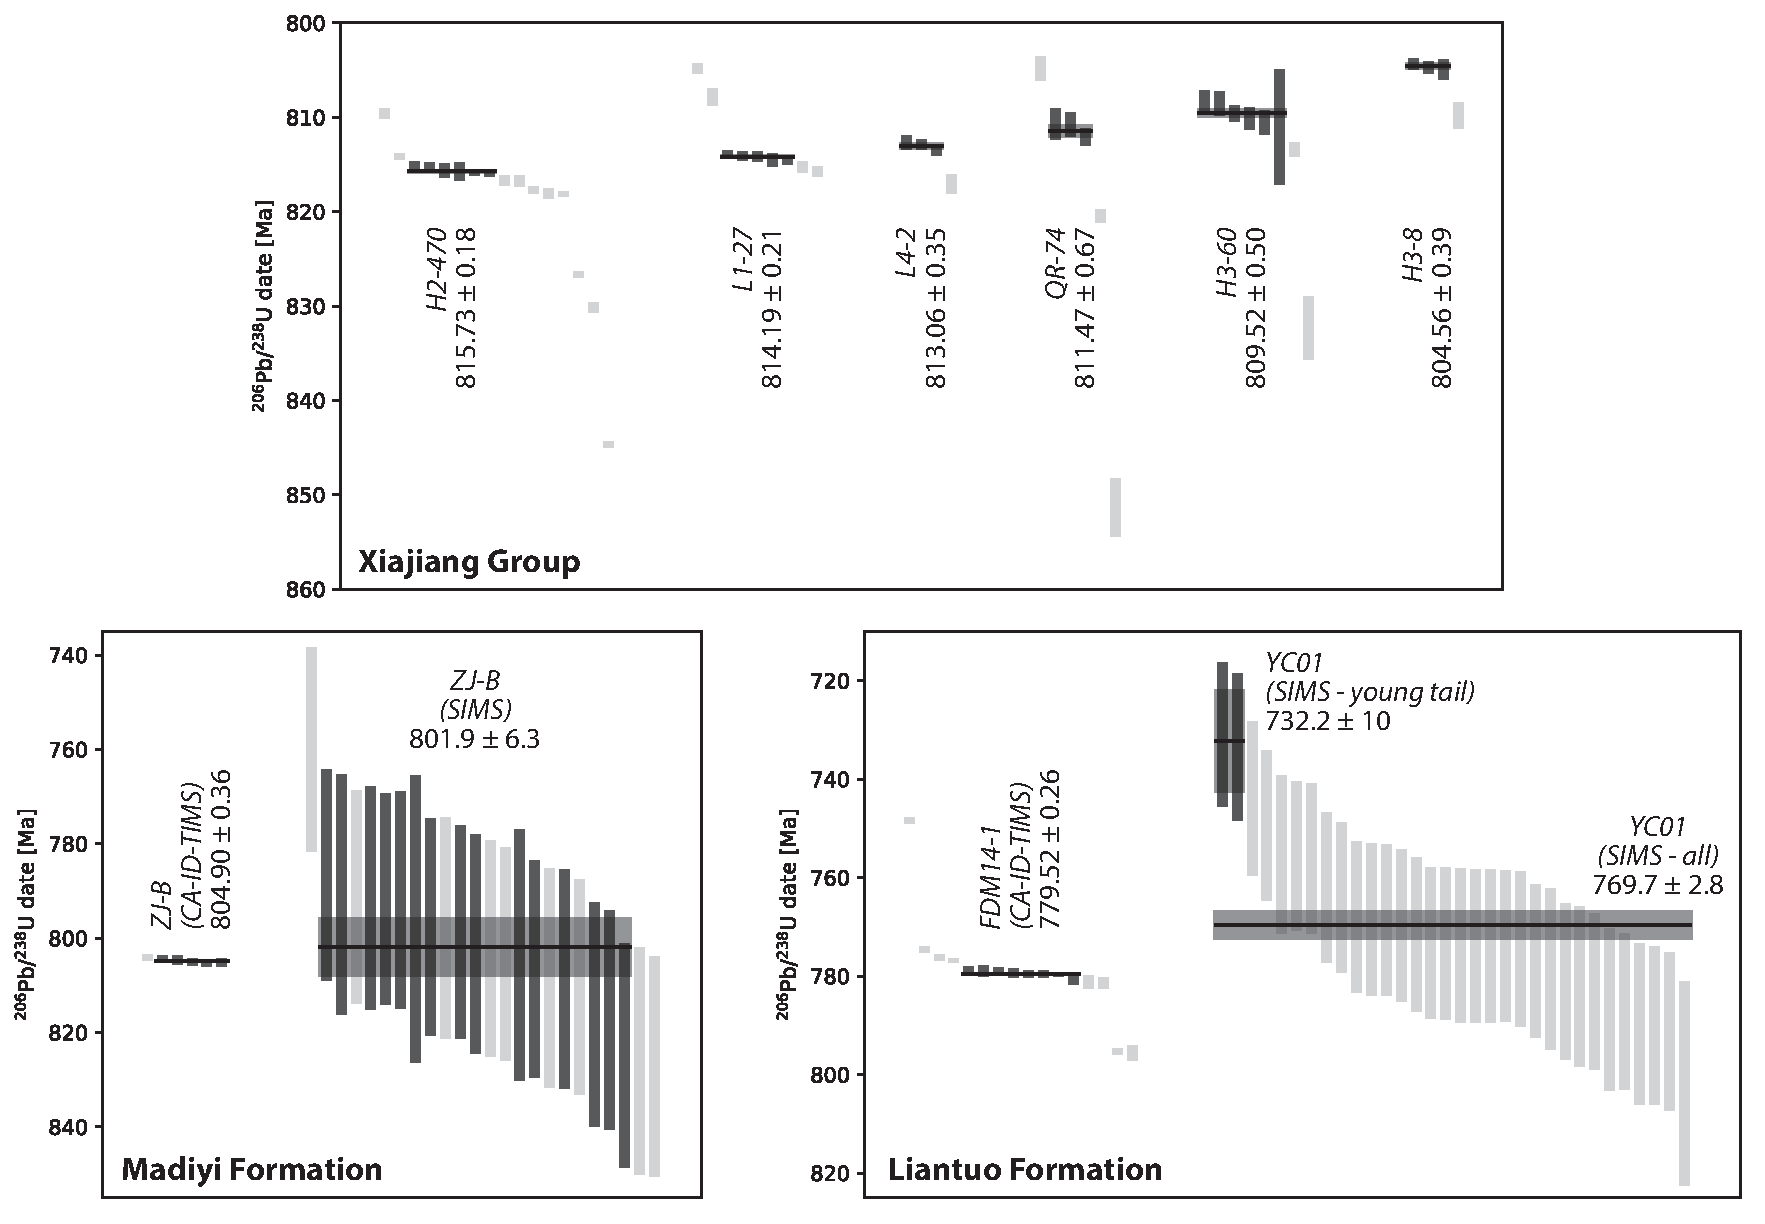
\includegraphics[width=\textwidth]{figures/Xiajiang/zircons.pdf}
    \caption[2$\sigma$ uncertainty of CA-ID-TIMS U-Pb dates for zircons analyzed in this study.]{2$\sigma$ uncertainty of CA-ID-TIMS U-Pb dates for zircons analyzed in this study. The previously reported SIMS dates for sample ZJ-B of the Madiyi Formation \citep{Xian2020a} and sample YC01 of the Liantuo Formation \citep{Lan2015a} are also shown. For sample YC01, we show the weighted mean dates that result from isolating the two youngest zircons (as is preferred in \citealp{Lan2015a}) and from including all of the zircons. Solid vertical bars indicate zircons that are included in the calculation of the weighted mean date. Faded vertical bars indicate zircons interpreted to have been inherited or affected by Pb or U loss, and are excluded in the calculation of the weighted mean date. Measurement data are and concordia diagrams are shown in the Supporting Information.}
    \label{fig:zircons}
\end{figure}

U-Pb zircon secondary ion mass spectrometry (SIMS) and laser ablation inductively coupled plasma mass spectrometry (LA-ICP-MS) analyses can be conducted relatively rapidly and are often utilized to determine the age of tuff samples. However, U-Pb determinations using SIMS are significantly less precise than that measured using CA-ID-TIMS and are subject to an U-Pb calibration correction that contributes additional uncertainty. This single data point imprecision makes it difficult to recognize real age variation within a sampled population (due to either analyses of domains with Pb loss and/or older zircon). As a result, isotope ratios measured using SIMS can be affected by Pb loss that cannot be identified at the precision of SIMS, which can bias SIMS-derived weighted mean dates toward younger ages. Conversely, deriving a weighted mean from a non-single age population (with variation not resolvable by the single data point analyses) can bias the interpreted age towards being too old. An additional issue in the interpretation of microbeam U-Pb geochronology is that there are dates in the literature where the youngest dates are deconvolved from a larger age population to derive a weighted mean that approximates the ages of eruption. Calculating a weighted mean from the `young tail' for a distribution of imprecise dates could result in a date that is too young either due to Pb loss in these grains or simply through arbitrary grouping of the youngest dates in a low precision normal distribution of dates. Such a bias could explain calculated SIMS dates from pre-Sturtian strata that are younger than ca. 717~Ma in South China (e.g. \citealp{Lan2015a}) and in practice requires other independent information to defend the interpretation. In addition to the issues surrounding age interpretations, microbeam U-Pb dates require consideration of the U/Pb calibration uncertainty that is typically 1--2\% and is a limiting uncertainty.

The chemical abrasion step of the CA-ID-TIMS method has been developed to effectively remove (i.e. leach) the analyses of radiation-damaged zones of zircon grains, which are most likely to suffer Pb loss, prior to analysis \citep{Mattinson2005a}. This technique is not perfect -- depending on the nature of the material being analysed (U content, zonation patterns), for some samples a proportion of analyses suffering Pb-loss may still persist. The higher-precision of the CA-ID-TIMS single data points often reveals age complexity with excess variance ascribed to geological age variation and residual Pb-loss.

Evaluating a hypothesis such as the Bitter Springs Stage TPW hypothesis requires precise age constraints on poles. The SIMS dates prevalent in the literature could have true age uncertainty well beyond the weighted mean uncertainty, particularly if the assumptions made are incorrect (i.e. a single age population, no Pb-loss) in addition to the calibration uncertainty. As a result, it is essential to develop CA-ID-TIMS dates in order to have high-precision age constraints on paleomagnetic poles.

We developed U-Pb CA-ID-TIMS ages from zircon for six tuff samples collected from the Xiajiang Group in the Fanjingshan region (Figs. \ref{fig:stratigraphic-sections} and \ref{fig:zircons}; Table \ref{tab:SChina-geochronology}). For each of these ash layers we make a subjective age interpretation based upon the U-Pb zircon data combined with information about the general nature of the materials. Five tuffs from the lower and middle Xiajiang Group yield dates ca. 816--810~Ma, and one tuff from near the top of the Xiajiang Group in the Hongzixi section yields a younger date of ca. 805~Ma. Within $\sim$100~m of this youngest tuff, a major unconformity separates ca. 805~Ma sediments of the Xiajiang Group with \textless717~Ma Sturtian Snowball Earth glacial deposits \citep{Bowring2007a, Macdonald2010a, MacLennan2018a, Lan2020a}.

Prior to this study, age constraints on Tonian paleomagnetic poles from the Madiyi and Liantuo formations were based on U-Pb SIMS analyses. In order to improve the precision of these age constraints, as well as evaluate whether they might be biased toward younger ages, we developed new age constraints for these poles using U-Pb CA-ID-TIMS. These new CA-ID-TIMS age constraints supersede the previous SIMS age constraints.

The tuff associated with the paleomagnetic pole for the Madiyi Formation in the Hunan province (sample ZJ-B of \citealp{Xian2020a}) is within the 12~m thick succession of the Madiyi Formation from which the paleomagnetic data were developed. A U-Pb zircon SIMS date of 801.9$\pm$6.3~Ma was reported for the tuff in \citet{Xian2020a}. The new CA-ID-TIMS data from five zircons result in a weighted mean $^{206}$Pb/$^{238}$U date of 804.90$\pm$0.36~Ma (Fig. \ref{fig:zircons}); Table \ref{tab:SChina-geochronology}). This date overlaps with the SIMS date of \citet{Xian2020a} within uncertainty and constrains the timing of the Madiyi Formation pole to higher precision.

The tuff associated with the paleomagnetic pole for the Liantuo Formation \citep{Evans2000a, Jing2015a} lies $\sim$15~m below the base of the stratigraphic interval which was sampled for paleomagnetic analysis in \citet{Evans2000a}, and is in the vicinity of a tuff that was previously dated at 748$\pm$12~Ma using SIMS (Fig. S5; \citealp{Ma1984a}). The new CA-ID-TIMS data from eight zircons result in a weighted mean $^{206}$Pb/$^{238}$U date of 779.52$\pm$0.26~Ma -- $\sim$20~m.y. older than the maximum reported uncertainty of the SIMS-derived date (Fig. \ref{fig:zircons}; Table \ref{tab:SChina-geochronology}).

\section{Discussion}

\subsection{Tectonic Setting}

The South China craton consists of two distinct tectonic blocks, the Yangtze and Cathaysia blocks, separated by the Jiangnan Orogen (Fig. \ref{fig:geologic-maps}). However, the depositional setting of sedimentary units in the Jiangnan Orogen as well as the tectonic context of the intrusive units and deformation found throughout the orogen continues to be debated in the literature. A widely-adopted model proposed that the Fanjingshan Group (and equivalent strata) was deposited in a Grenvillian (ca. 1.3--0.9~Ga) arc-related basin on the Yangtze block as the oceanic crust formerly separating the Yangtze and Cathaysia blocks subducted under the Yangtze block (e.g. \citealp{Li2002a, Li2009b}). In this model, deformation of the Fanjingshan Group was interpreted to reflect collision of the Yangtze and Cathaysia blocks as the supercontinent Rodinia came together around South China ca. 1.0--0.9~Ga, with Laurentia on the Cathaysia-side of South China and Australia on the Yangtze-side (i.e. the Missing Link model, as shown in Figure \ref{fig:Rodinia-models}). The model then proposes that later Tonian (ca. 850--750~Ma) magmatism in the Jiangnan Orogen is associated with a mantle superplume that initiated the break up of Rodinia (e.g. \citealp{Li2003a, Li2009b}). In this scenario, the Xiajiang Group (and equivalent strata) is interpreted to have been deposited within a failed intra-continental rift basin between the Yangtze and Cathaysia blocks as Australia, South China, and Laurentia rifted apart.

Geochronologic and geochemical data initially appeared to support this Missing Link model (e.g. \citealp{Li2002a, Li2003a, Li2009b}), and consequently many Neoproterozoic paleogeographic models adopted it (e.g. \citealp{Li2008a}). However, subsequent geochronologic, geochemical, and paleomagnetic data introduce new constraints that are difficult to reconcile with this model.

The timing of Yangtze and Cathaysia block collision represented by the Jiangnan Orogen can no longer be considered to be coeval with the ca. 1080 to 980~Ma Grenvillian Orogen. U-Pb LA-ICP-MS geochronologic constraints from the tuffs, sedimentary rocks, and sills of the Fanjingshan Group \citep{Zhao2011a, Wang2012d, Gao2014a} indicate that deformation of the group occurred after ca. 830~Ma. Our new U-Pb CA-ID-TIMS results constrain initiation of Xiajiang Group deposition, and therefore termination of Fanjingshan Group deformation, to have occurred by 815.73$\pm$0.18~Ma (Fig. \ref{fig:stratigraphic-sections}). The interpretation that the Jiangnan Orogeny, and the associated deformation of the Fanjingshan Group, was the result of collision between the Yangtze and Cathaysia blocks gains support from the geochemistry and geochronology of the igneous rocks of the Jiangnan Orogen that are indicative of a supra-subduction, volcanic arc setting \citep{Cawood2013a, Cawood2017a}.

The Fanjingshan Group is dominated by siliciclastic sediments and also contains horizons of volcanic rocks including pillow basalts \citep{Zhou2009a}. These units were intruded by ca. 830~Ma mafic sills with geochemical signatures consistent with subduction-related magmatism \citep{Wang2014a} as well as 835$\pm$5~Ma (U-Pb SIMS) felsic intrusive rocks (Fig. \ref{fig:geologic-maps}B; \citealp{Gao2011a}). Both fore-arc \citep{Zhao2011a} and retro/back-arc \citep{Lin2016a, Yao2019a} settings have been interpreted for the Fanjingshan Group deposition. However, fore-arc settings are typically cold and amagmatic, and consequently we prefer a syn-collisional retro-arc foreland model with ultramafic magmatism associated with slab-breakoff. In either model, the Fanjingshan Group is deposited and intruded in an arc-related basin as the oceanic crust formerly separating the Yangtze and Cathaysia blocks subducted under the Yangtze block \citep{Lin2016a}. As Yangtze and Cathaysia (or at least a portion of Cathaysia) collided between ca. 830~Ma and 815.73$\pm$0.18~Ma, sedimentary rocks of the Fanjingshan Group were folded, uplifted, and eroded. Following this deformation and the development of an erosional unconformity, subsidence enabled deposition of the overlying Xiajiang Group. Taken together, these data constrain the collision of the Yangtze and Cathaysia blocks to have occurred between ca. 830~Ma and 815.73$\pm$0.18~Ma, not ca. 1000 to 900~Ma as is proposed in the Missing Link model implemented in \citet{Li2008a}.

In addition to this evidence of Tonian convergence between the Yangtze and Cathaysia blocks, the record of the northwest Yangtze block indicates a convergent tectonic setting in the Tonian that extended into the Cryogenian. Geochronologic and geochemical constraints from the Panxi-Hannan Belt (Fig. \ref{fig:geologic-maps}) indicate that arc-related magmatism was occurring in that belt ca. 870--706~Ma \citep{Dong2012a}, and therefore that the northwestern margin of the Yangtze block was an active margin throughout the time that Rodinia is hypothesized to have been a coherent supercontinent. This arc-related magmatic activity associated with subduction along the northwestern margin of the Yangtze block is the likely source for the ashes that formed the tuffs within the Xiajiang Group that we have targeted for geochronology (Fig. \ref{fig:stratigraphic-sections}).

Finally, paleomagnetic constraints indicate that South China was at high latitudes throughout the late Tonian (discussed further in \textit{Tonian APWP of South China}) rather than at low-latitudes as would be required by the Missing Link model (discussed further in \textit{South China and Rodinia}; Fig. \ref{fig:Rodinia-models}). Additionally, the paleomagnetic data suggests that the Panxi-Hannan Belt lay from the east to the north relative to the Fanjingshan region in reconstructed coordinates during the time of Xiajiang Group deposition (ca. 815--800~Ma; Fig. \ref{fig:SChina-APWP}). At these high latitudes, the prevailing winds are polar easterlies, which is consistent with the idea that the ashes that formed the tuffs within the Xiajiang Group were transported from the Panxi-Hannan Belt \citep{Hildebrand1988a}.

Together, these constraints are inconsistent with South China being within the interior of a stable supercontinent during the Tonian. Instead, they indicate a convergent setting with the northwestern margin of the Yangtze block being an active margin into the Cryogenian rather than being juxtaposed against a conjugate continent. Therefore, the data are more compatible with South China on the periphery of Rodinia or disconnected from it entirely (Fig. \ref{fig:Rodinia-models}).

The tectonic setting of the basin in which the Xiajiang Group (and equivalent strata) was deposited is commonly interpreted as a failed intra-continental rift basin \citep{Zhang2019c}, potentially associated with the hypothesized mantle superplume that initiated the break up of Rodinia \citep{Li2003a, Li2009b}. However, this basin development framework is rooted in a tectonic setting interpretation that would have South China within the interior of a supercontinent undergoing break-up --- a setting that is inconsistent with available constraints. Rather, any basin development model needs to honor the following:

\begin{itemize}
    \item There was a geologically short interval (ca. 15~m.y.) between the orogenesis that deformed the Fanjingshan Group and the subsidence that enabled deposition of the Xiajiang Group.
    \item There was an active margin along the northwestern margin of the Yangtze block at the time of Xiajiang Group subsidence. This margin is the likely source of the tuffs throughout the Xiajiang Group stratigraphy.
    \item The site of Xiajiang Group deposition must have been folded, uplifted, and eroded prior to subsidence.
    \item Subsidence rates were initially quite high as evidenced by the rapid sediment accumulation rates in the Xiajiang Group. These high subsidence rates led to the deep-water setting of the Xiajiang Group sediments.
    \item While some strata could be missing through glacial erosion, the duration of missing time ($\sim$90~m.y.) in the ca. 805 and 717~Ma pre-Sturtian unconformity suggests limited sediment accumulation in the pre-Sturtian interval relative to the thick ca. 815 to 805~Ma succession.
\end{itemize}

The Nanhua Basin into which the Xiajiang Group was deposited formed inland from the Panxi-Hannan Belt \citep{Cawood2017a}. Based on the interpretation that the Panxi-Hannan Belt was an active arc at the time of Xiajiang Group deposition, \citet{Qi2019a} argued that Nanhua Basin formation was the result of back-arc extension. Importantly, the timing of deposition of the Xiajiang Group coincides with the initiation of  back-arc extension in the Panxi-Hannan arc \citep{Dong2012a}. Back-arc extension provides a mechanism to explain regional extension and subsidence in the region of the Jiangnan suture. Furthermore, given that back-arc basin formation is the result of the combined driving mechanisms of surface kinematics and dynamic mantle flow \citep{Sdrolias2006a}, it can lead to both rapid and transient subsidence. Geologic observations in more recent back-arcs have been interpreted to indicate significant back-arc extension in regions where lithosphere has been thickened through orogenesis \citep{Gogus2015a}. Numerical modeling has shown that post-orogenic lithosphere removal (such as that occurring as a result of delamination) in continental back-arc settings can lead to large-scale subsidence \citep{Gogus2015a}. This mechanism could explain the transition at the site of Xiajiang Group deposition from folding, uplift, and erosion in the Jiangnan Orogen as Yangtze collided with Cathaysia between ca. 830~Ma and 815.73$\pm$0.18~Ma, to Nanhua Basin subsidence as a back-arc basin formed. The Nanhua Basin is therefore best interpreted as a polyphase basin wherein this Tonian subsidence was followed by Cryogenian and Ediacaran subsidence potentially as the result of other mechanisms. The tuffs found throughout the Xiajiang Group stratigraphy are the result of the arc on the northwestern margin of the Yangtze block that was active throughout deposition, both driving subsidence through back-arc extension and contributing ashes via the prevailing polar easterly winds that enable us to develop geochronologic constraints.

\subsection{Tonian APWP of South China}

\begin{table}[h!]
\caption[Neoproterozoic paleomagnetic poles for South China.]{Neoproterozoic paleomagnetic poles for South China.}
\vspace{0.25cm}
\resizebox{\linewidth}{!}{
	\begin{tabular}{lllccccccllc}
	\hline
	\textbf{pole} & \textbf{nominal age (Ma)} & \textbf{age method} & \textbf{site lat.} & \textbf{site lon.} & \textbf{pole lat.} & \textbf{pole lon.} & \textbf{A$_{95}$} & \textbf{f} & \textbf{pole ref.} & \textbf{age ref.} & \textbf{note} \\\\
	Yanbian dikes & 824$\pm$6 & SIMS & 26.9 & 101.5 & 45.1 & 130.4 & 19.0 & 1.0 & \citet{Niu2016a} & \citet{Niu2016a} & (2) \\
    Xiaofeng dikes & 821.64$\pm$0.2 & CA-ID-TIMS & 31.0 & 111.2 & 26.1 & 82.1 & 14.6 & 1.0 & \citet{Jing2019a} & \citet{Wang2016b} & (3) \\
    Xiajiang Group & 816--810 & CA-ID-TIMS & 27.9 & 108.8 & 42.7 & 104.0 & 8.1 & 0.6 & this study & this study & - \\
	Madiyi Formation & 804.90$\pm$0.99 & CA-ID-TIMS & 27.5 & 109.6 & 34.7 & 82.0 & 6.7 & 0.6 & \citet{Xian2020a} & this study & (4) \\
    Chengjiang Formation & 799.5$\pm$8.4 & SIMS & 25.1 & 102.4 & 29.7 & 75.3 & 7.9 & 0.6 & \citet{Jing2019a} & \citet{Jing2019a} & (5) \\
    Liantuo Formation & $\leq$779.52$\pm$0.92 & CA-ID-TIMS & 30.8 & 111.1 & 19.6 & 144.4 & 4.2 & 0.6 & \citet{Jing2015a} & this study & (5) \\
	\hline
	\end{tabular}}

\scriptsize
\flushleft \emph{Notes:} \\
(1) \textbf{f} is the flattening factor, where f=1 indicates no inclination shallowing and f=0 indicates a completely flattened direction.\\
(2) Located within mobile belt.\\
(3) Pole recalculated after \citet{Li2004a}.\\
(4) Pole converted from specimen to site mean in this study.\\
(5) Pole converted from specimen to site mean and inclination correction applied in this study.\\
\label{tab:South-China-poles}
\end{table}

\begin{figure}[h!]
    \centering
    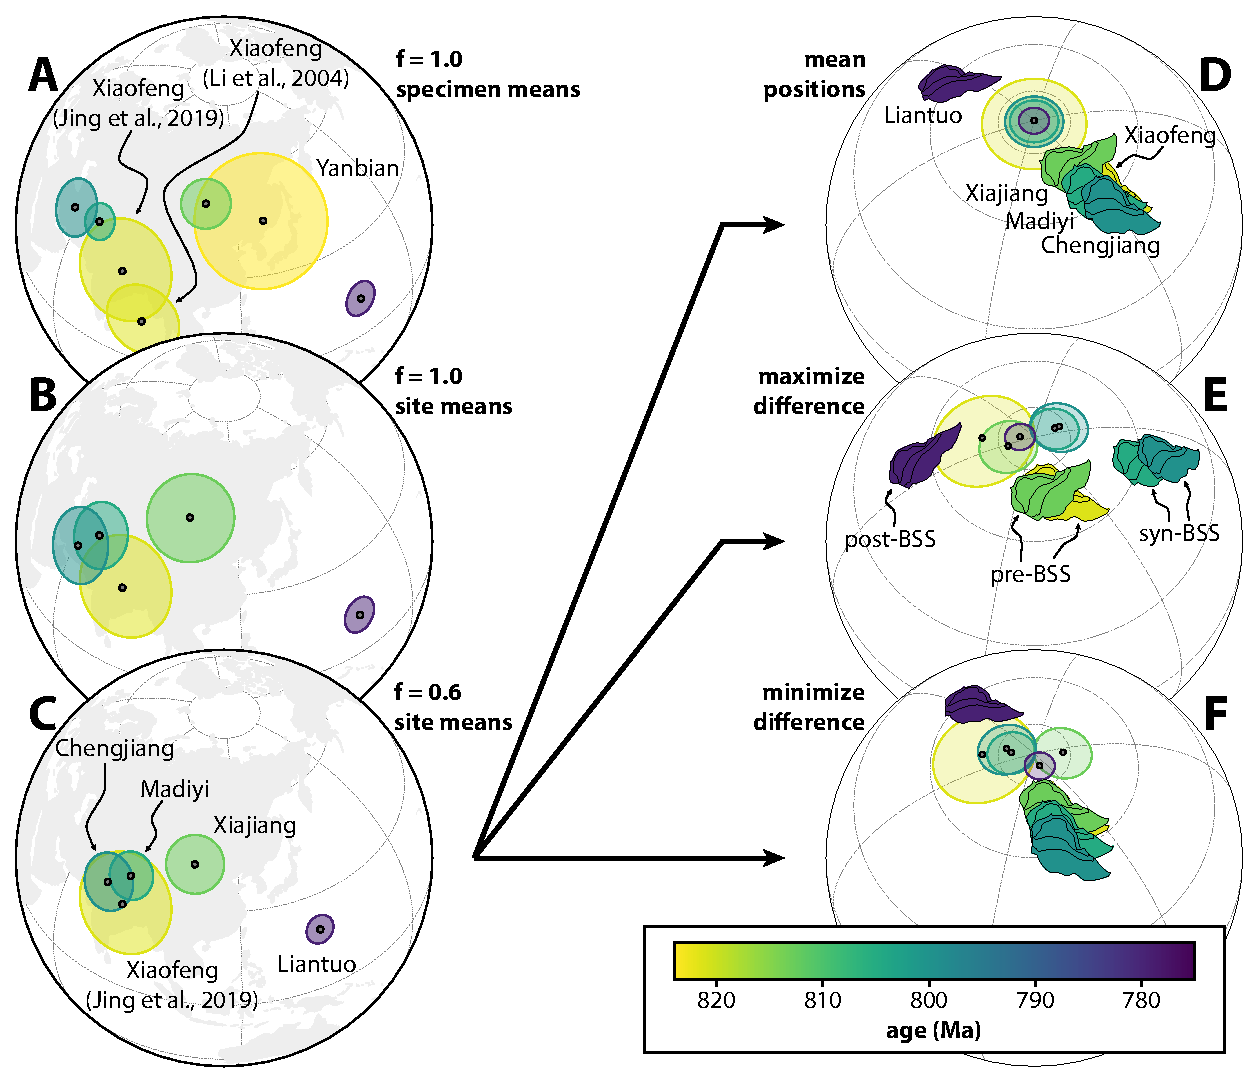
\includegraphics[width=\textwidth]{figures/Xiajiang/SChina-APWP.pdf}
    \caption[Tonian apparent polar wander paths and paleogeographic models for South China.]{Tonian apparent polar wander paths (APWPs) and paleogeographic models for South China. \textbf{A)} APWP using all available paleomagnetic poles. Poles derived from sedimentary rocks are shown as specimen means without an inclination correction (Table \ref{tab:South-China-poles}). \textbf{B)} APWP excluding the Yanbian dikes pole. Poles derived from sedimentary rocks are shown as site means without an inclination correction. \textbf{C)} Our preferred APWP excluding the Yanbian dikes pole and using site mean poles from sedimentary rocks with an inclination correction ($f=0.6$). \textbf{D)} Paleogeographic model based on the preferred APWP in C. South China is reconstructed using the means of the poles. \textbf{E)} Paleogeographic model based on the preferred APWP with South China reconstructed to maximize the difference in position between the pre-, syn-, and post-Bitter Springs Stage (BSS) poles as permitted by the A$_{95}$ uncertainties. \textbf{F)} Paleogeographic model based on the preferred APWP with South China reconstructed to minimize the difference in position permitted by the A$_{95}$ uncertainties of all poles.}
    \label{fig:SChina-APWP}
\end{figure}

With the exception of the highest ash sample in the Hongzixi section, all dated ash samples from the Xiajiang Group of the Fanjingshan region yield an age of ca. 816--810~Ma (Fig. \ref{fig:stratigraphic-sections}). Furthermore, the high temperature components in all sites record similar directions (Fig. \ref{fig:site-means}). We therefore take the parsimonious interpretation that variability in the high temperature component between specimens/sites is largely recording short time-scale secular variability in the magnetic field, and therefore develop a single paleomagnetic pole from the mean direction of the high temperature component from all sites (Fig. \ref{fig:site-means}). Based on the geochronologic constraints (Fig. \ref{fig:stratigraphic-sections}), we assign a nominal age to this pole of 813$\pm$3~Ma. However, we discuss the possibility of multiple poles being recorded in the Xiajiang Group below.

This new pole can be combined with existing Neoproterozoic paleomagnetic poles for South China (summarized in Table \ref{tab:South-China-poles}) to develop an apparent polar wander path (APWP). There are complications associated with the interpretation of these poles and their assigned ages and we will discuss each in turn.

The Yanbian dikes pole \citep{Niu2016a} was obtained from a deformed region on the western-most margin of the South China craton that experienced vertical axis rotation during the Cenozoic collision of India with Asia. The magnitude of this vertical axis rotation was estimated to be 5.3$\pm$3.0\degrees based on paleomagnetic data from Pliocene sedimentary rocks in the region \citep{Zhu2008a}, and \citet{Niu2016a} applied a 5\degrees vertical axis rotation correction to their Yanbian dikes pole. However, the vertical axis rotation correction may be as little as 2.3\degrees or as high as 8.3\degrees at the 95\% confidence level \citep{Zhu2008a}. The Yanbian dikes may also have experienced pre-Pliocene vertical axis rotation. Furthermore, no tilt-correction was applied to the majority of the directions obtained from the Yanbian dikes, despite observations that the dikes exhibit dips that range from 43\degrees to vertical \citep{Niu2016a}. Finally, the Yanbian dikes pole is inconsistent with the Xiaofeng dikes pole (Fig. \ref{fig:SChina-APWP}A) despite the similar age of these two poles. Given these complications, we exclude the Yanbian dikes pole as a constraint in our preferred Tonian South China APWP (Fig. \ref{fig:SChina-APWP}C).

The Xiaofeng dikes pole has had both its direction and age revised since its initial publication in \citet{Li2004a}. \citet{Jing2019a} recognized that a subset of the dikes that were used to obtain the Xiaofeng dikes pole are located between two faults and have paleomagnetic directions that may have been rotated relative to the rest of the dikes. Therefore, to account for the possibility of vertical axis rotation affecting this subset of dikes, \citet{Jing2019a} recalculated the Xiaofeng dikes pole by excluding them. The resulting pole is closer to the other ca. 820-800~Ma poles for South China. In addition, the Xiaofeng dikes were originally dated to 802$\pm$10~Ma based on U-Pb SIMS analyses on zircon from the dikes \citep{Li2004a}. When zircon from these dikes were reanalyzed at higher precision using CA-ID-TIMS, their age was revealed to be significantly older (821.64$\pm$0.2~Ma; \citealp{Wang2016b}). This revised age constraint for the Xiaofeng dikes pole is utilized here (Table \ref{tab:South-China-poles}; Fig. \ref{fig:SChina-APWP}).

The previous age constraint on the Madiyi Formation pole of 801.9$\pm$6.3~Ma was also developed using U-Pb SIMS measurements on zircon from a tuff within the section where the paleomagnetic data were developed \citep{Xian2020a}. Our new CA-ID-TIMS date of 804.90$\pm$0.36~Ma is within the uncertainty of this SIMS date and provides a higher precision age constraint on the age of the pole (Fig. \ref{fig:zircons}) which supersedes the previous age and is utilized here (Table \ref{tab:South-China-poles}; Fig. \ref{fig:SChina-APWP}).

The paleomagnetic pole for the upper Liantuo Formation has long been an important constraint for the Neoproterozoic paleogeography of South China \citep{Evans2000a}. The Liantuo Formation unconformably overlies the Huangling granite suite for which U-Pb SIMS dates of 863$\pm$9, 844$\pm$10, and 842$\pm$10~Ma have been developed \citep{Wei2012a}. These granites are intruded by the 821.64$\pm$0.2~Ma Xiaofeng dikes \citep{Wang2016b}. The Liantuo Formation is unconformably overlain by Cryogenian glacial deposits. The age assigned to the Liantuo Formation pole has varied in the literature. When a paleomagnetic pole from the formation was first reported in \citet{Evans2000a}, it was assigned an age of 748$\pm$12~Ma based on an U-Pb SIMS date on a tuff $\sim$15~m below the base of the stratigraphic interval that was sampled for paleomagnetic analysis (\citealp{Ma1984a}; Fig. S5). When this paleomagnetic pole was updated in \citet{Jing2015a} with the addition of paleomagnetic data from additional sites to the southwest of the stratigraphic section sampled in \citet{Evans2000a}, its age was interpreted to be ca. 720~Ma based on U-Pb SIMS dates on tuffs within the upper 20~m of the Liantuo Formation across the Three Gorges Area \citep{Lan2015a}. A challenge with these U-Pb SIMS dates is that there is a distribution of dated grains around a peak of ca. 780 to 770~Ma that includes sparse younger dates (Fig. \ref{fig:zircons}; \citealp{Lan2015a}). In \citet{Lan2015a}, these younger dates are interpreted as the eruptive age of the tuffs, but it is possible that these grains are biased young. Ambiguity associated with correlation of the Liantuo Formation with possibly equivalent stratigraphy adds further complexity to the interpretation of geochronologic constraints on the Liantuo Formation. For example, zircons from a tuffaceous siltstone $\sim$25~m below Sturtian glacial deposits in the Gongdong Formation of northern Guangxi, which is often interpreted to be a deeper water equivalent to the Liantuo Formation \citep{Wang2003a, Pi2016a}, yield a weighted mean CA-ID-IRMS date of 720.16$\pm$1.40~Ma \citep{Lan2020a}. If this interpretation that the Gongdong Formation correlates to the Liantuo Formation is correct, it suggests that, at least in some parts of the Nanhua Basin, sediments as young as ca. 720~Ma are preserved. On the other hand, if the two formations are not correlative, then the CA-ID-IRMS date of 720.16$\pm$1.40~Ma \citep{Lan2020a} does not place any geochronologic constraints on the Liantuo Formation.

We have developed a new CA-ID-TIMS date of 779.52$\pm$0.26~Ma for a tuff in the Liantuo Formation at the same location studied by \citet{Ma1984a} close to the section sampled for paleomagnetic analyses by \citet{Evans2000a}. Similar to the updated Xiaofeng dikes geochronology, this date is appreciably older than interpretations based on the previous SIMS U-Pb dates. While the $\sim$15~m of stratigraphy between the tuff and the paleomagnetic data of \citet{Evans2000a} could represent significant time, the similar lithologies throughout the interval (fine to medium sandstone interbedded with siltstone; Fig. S5) suggests conformable deposition. Therefore, the age of the tuff is likely to be similar in age to the sedimentary rocks from which the paleomagnetic data were derived and unlikely to be tens of millions of years older. Nevertheless, without further high-precision geochronologic constraints from the Liantuo Formation at or above the stratigraphy from which the paleomagnetic pole was derived, the possibility remains that the Liantuo Formation paleomagnetic pole post-dates 779.52$\pm$0.26~Ma. Thus, we suggest the age of the Liantuo Formation and its pole is close to 780~Ma and that the Liantuo Formation is not correlative to the ca. 720~Ma Gongdong Formation, which is preserved conformably below Cryogenian glacial deposits in a deeper-water setting \citep{Lan2020a}.

The existing date of 799.5$\pm$8.4 Ma for the Chengjiang Formation pole was also developed using SIMS (Table \ref{tab:South-China-poles}). As evidenced for the Xiaofeng dikes and the Liantuo Formation, when SIMS-derived ages are re-investigated through CA-ID-TIMS, the result can be a significantly different date. Therefore, the accuracy of the SIMS-derived dates for the Chengjiang Formation pole remains uncertain.

The Xiajiang Group paleomagnetic pole developed in this study is calculated as a site mean (i.e. the mean of the means of specimen directions for each site; Fig. \ref{fig:site-means}). However, the Chengjiang and Madiyi poles are reported in \citet{Jing2019a} and \citet{Xian2020a} as specimen means (i.e. the mean of specimen directions across all sites). While both methods can be justified for sedimentary rocks, the specimen mean direction leads to paleomagnetic poles with smaller $A_{95}$ uncertainty ellipses due to the larger number of directions used to obtain the mean which has the potential to underestimate the uncertainty. We recalculate the paleomagnetic poles for the Chengjiang and Madiyi formations as site means, to be consistent with the methodology used to develop our Xiajiang Group pole (Figs. \ref{fig:SChina-APWP}B and \ref{fig:SChina-APWP}C).

An inclination correction has been applied to the paleomagnetic pole obtained from the Xiajiang Group in this study. Similarly, an inclination correction was applied to the pole obtained from the Madiyi Formation \citep{Xian2020a}. Given that the poles from the Chengjiang and Liantuo formations are also derived from the hematite-held magnetization of similar siliciclastic sedimentary rocks, we apply the same inclination correction ($f=0.6$) to these poles as that applied to the Xiajiang Group and Madiyi Formation poles (Fig. \ref{fig:SChina-APWP}C). Given potential variability in inclination shallowing, the flattening could vary from this value which is an additional source of uncertainty.

The Xiaofeng dikes and the inclination-corrected Madiyi and Chengjiang poles all overlap within uncertainty, and the Xiajiang Group records a distinct, but similar, position as well (Fig. \ref{fig:SChina-APWP}). Together, these poles constrain South China to have been in a roughly stable position at high latitudes ($\gtrsim$60\degrees) ca. 820--800~Ma (Figs. \ref{fig:SChina-APWP} and \ref{fig:centroid-paleolatitudes}). The Liantuo Formation pole also constrains South China to be at high latitudes, although with a different orientation to the ca. 820--800~Ma position (Figs. \ref{fig:SChina-APWP} and \ref{fig:centroid-paleolatitudes}). The poles constrain South China to be at high latitudes in the latter half of the Tonian, likely drifting across the pole after ca. 805~Ma (Fig. \ref{fig:SChina-APWP}).

\subsection{South China and Rodinia}

\begin{table}[h!]
\caption[900-700~Ma paleomagnetic poles for cratons proximal to South China.]{900-700~Ma paleomagnetic poles for cratons proximal to South China.}
\vspace{0.25cm}
\resizebox{\linewidth}{!}{
	\begin{tabular}{lcccccclc}
	\hline
	\textbf{pole} & \textbf{nominal age (Ma)} & \textbf{site lat.} & \textbf{site lon.} & \textbf{pole lat.} & \textbf{pole lon.} & \textbf{A$_{95}$} & \textbf{ref.} & \textbf{grade} \\
	&&&&&&&& \\
	\textbf{Laurentia} &&&&&&&& \\
	Gunbarrel dikes & 778$^{+2}_{-2}$ & 44.8 & 248.7 & 9.1 & 138.2 & 12.0 & \citet{Eyster2019a} & B \\
	Uinta Mountain Group & 760$^{+6}_{-10}$ & 40.8 & 250.7 & 0.8 & 161.3 & 4.7 & \citet{Weil2006a} & B \\
	Carbon Canyon & 757$^{+7}_{-7}$ & 36.1 & 248.2 & -0.5 & 166 & 9.7 & \citet{Eyster2019a} & NR \\
	Carbon Butte/Awatubi & 751$^{+8}_{-8}$ & 35.2 & 248.5 & 14.2 & 163.8 & 3.5 & \citet{Eyster2019a} & NR \\
	Franklin event grand mean & 724$^{+3}_{-3}$ & 73.0 & 275.4 & 6.7 & 162.1 & 3.0 & \citet{Denyszyn2009a} & A \\
	&&&&&&&& \\
	\textbf{Svalbard} &&&&&&&& \\
	Lower Grusdievbreen Formation & 815$^{+5}_{-5}$ & 79.0 & 18.0 & 19.6 & 204.9 & 10.9 & \citet{Maloof2006a} & B \\
	Upper Grusdievbreen Formation & 802$^{+8}_{-7}$ & 78.9 & 18.2 & -1.1 & 252.6 & 6.2 & \citet{Maloof2006a} & B \\
	Svanbergfjellet Formation & 785$^{+5}_{-5}$ & 78.5 & 18.0 & 25.9 & 226.8 & 5.8 & \citet{Maloof2006a} & B \\
	&&&&&&&& \\
	\textbf{Siberia} &&&&&&&& \\
	Kitoi Cryogenian dikes & 758$^{+4}_{-4}$ & 52.3 & 102.8 & 1.1 & 21.8 & 5.6 & \citet{Pisarevsky2013a} & A \\
	&&&&&&&& \\
	\textbf{Australia} &&&&&&&& \\
	Browne Formation & 855$^{+45}_{-45}$ & -25.0 & 123.8 & 44.5 & 141.7 & 6.8 & \citet{Pisarevsky2007a} & B \\
	Johnny's Creek siltstones & 760$^{+30}_{-30}$ & -24.0 & 133.5 & 15.8 & 83.0 & 13.5 & \citet{Swanson-Hysell2012a} & B \\
	Mundine Well dikes combined & 755$^{+3}_{-3}$ & -25.5 & 115.0 & 45.3 & 135.4 & 4.1 & \citet{Wingate2000a} & A \\
	&&&&&&&& \\
	\textbf{India} &&&&&&&& \\
	Malani Igneous Suite combined & 752$^{+18}_{-18}$ & 25.3 & 72.6 & 69.4 & 78.6 & 6.0 & \citet{Meert2013a} & A \\
	\hline
	\end{tabular}}

\scriptsize
\flushleft \emph{Notes:} \\
(1) \textbf{grade} is the quality of the pole as assessed by the Nordic Paleomagnetism Workshops \citep{Evans2021a}. `A' refers to poles that are considered to provide essential constraints given their high quality. `B'
refers to poles that are likely high quality, but retain some ambiguity about their age or direction. `NR' refers to poles that were not rated at the Nordic Paleomagnetism Workshops. \\
\label{tab:other-poles}
\end{table}

\begin{figure}[h!]
    \centering
    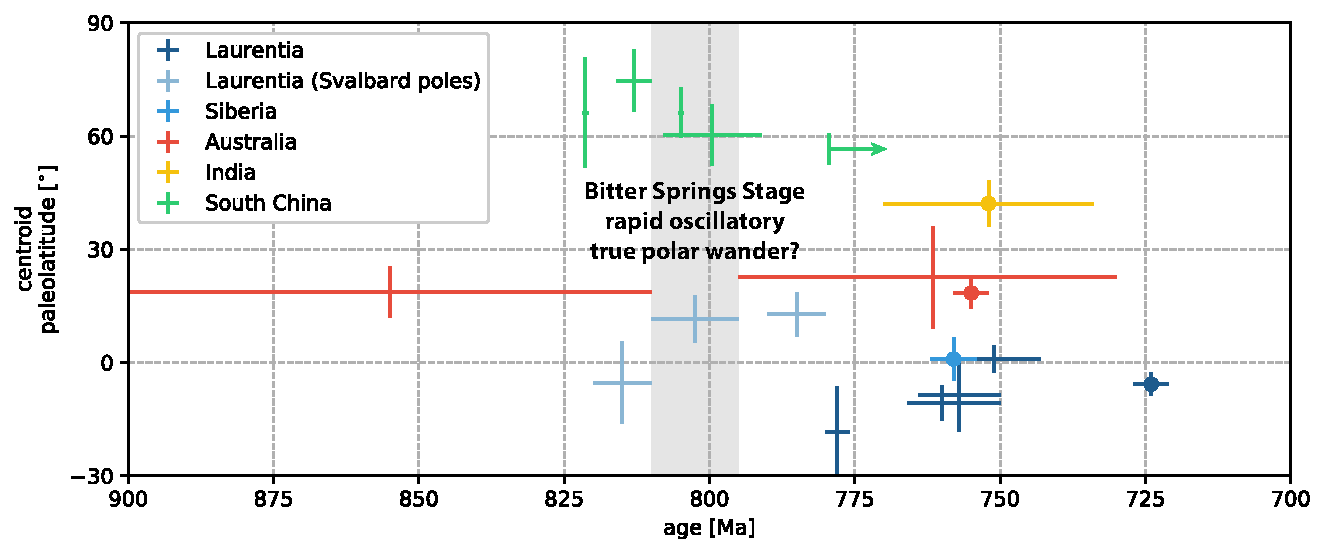
\includegraphics[width=\textwidth]{figures/Xiajiang/centroid-paleolatitudes.pdf}
    \caption[Paleolatitudes of points in the center of South China and other cratons implied by available paleomagnetic poles.]{Paleolatitudes of points in the center of South China and other cratons implied by available paleomagnetic poles shown with age and paleolatitude uncertainty (Tables \ref{tab:South-China-poles} and \ref{tab:other-poles}). The light blue `Laurentia (Svalbard poles)' are for the centroid of Laurentia reconstructed using Svalbard poles with Svalbard rotated back to Laurentia. Points with a circle in the center indicate paleomagnetic poles that were given an `A' rating by the Nordic Paleomagnetism Workshops. The grey bar indicates the timing of the ca. 810-795~Ma Bitter Springs Stage which is hypothesized to have been bracketed by rapid true polar wander rotations.}
    \label{fig:centroid-paleolatitudes}
\end{figure}

\begin{figure}[h!]
    \centering
    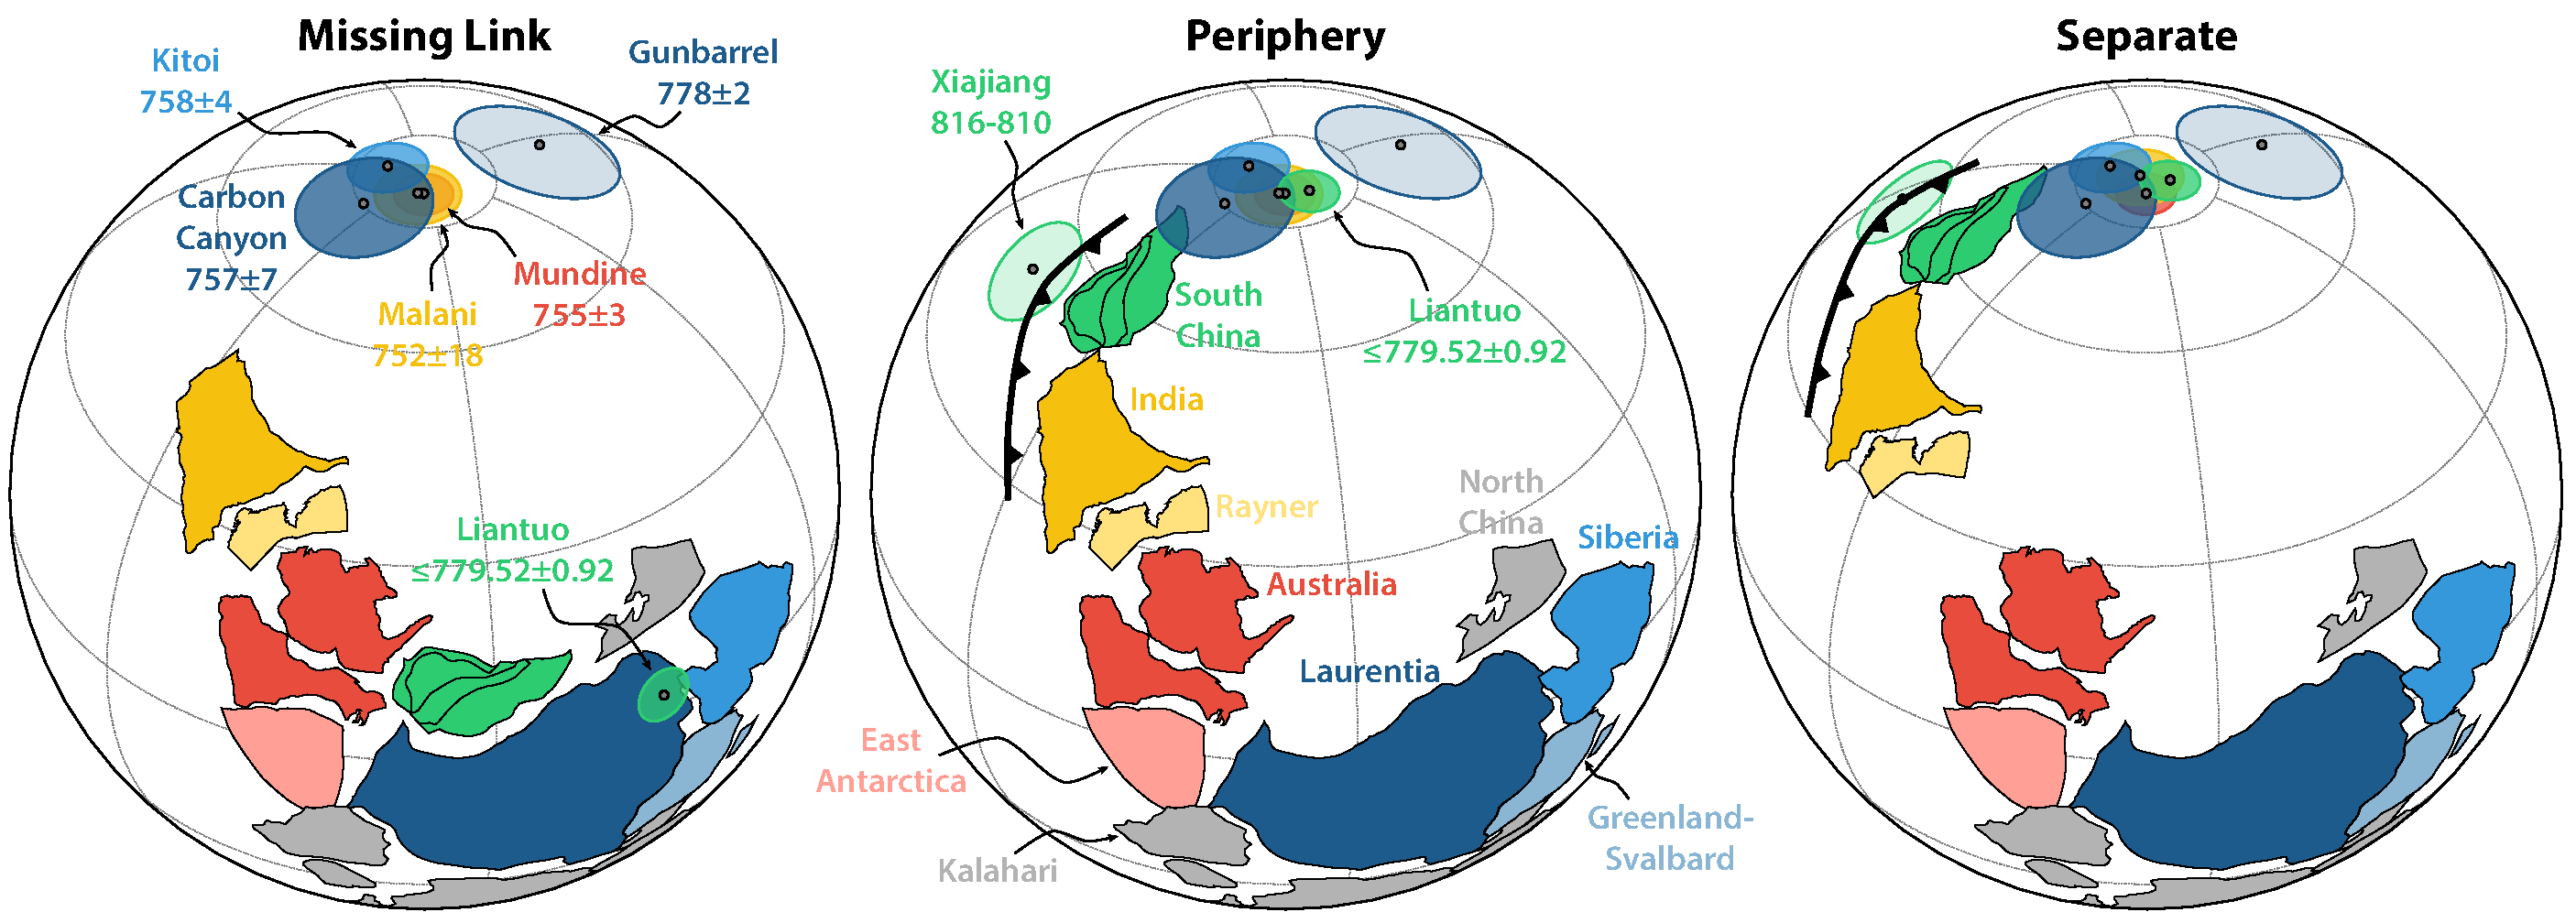
\includegraphics[width=\textwidth]{figures/Xiajiang/Rodinia-models.pdf}
    \caption[Paleogeographic reconstructions for Rodinia at 755~Ma.]{Paleogeographic reconstructions for Rodinia at 755~Ma. The Missing Link model places South China at low latitudes between Australia and Laurentia, which is inconsistent with both the paleomagnetic data as well as the tectonic context of South China. The Periphery model instead places South China at high latitudes connected to India, which satisfies the ca. 755~Ma and 780~Ma paleomagnetic data and allows for an active margin along the Panxi-Hannan Belt at this time. In order to satisfy ca. 821-805~Ma paleomagnetic data from South China, anticlockwise rotation of the entire Rodinia supercontinent from ca. 821-805~Ma to ca. 780~Ma is required in this Periphery model. The Separate model disconnects South China-India-Rayner from Rodinia. The Euler rotation parameters for South China relative to India in the Periphery and Separate models are (6.72\degrees N, 77.69\degrees E, 67.96\degrees). Blocks that are not directly relevant to the relationship between South China and Rodinia are shown in grey.}
    \label{fig:Rodinia-models}
\end{figure}

Connections between some of the cratons on the northern margin of Rodinia (present-day western margin of Laurentia) are reasonably well-established for the late Tonian (Fig. \ref{fig:Rodinia-models}). Siberia's long-lived ca. 1.7--0.7~Ga connection to the present-day northwestern margin of Laurentia is constrained by coeval paleomagnetic poles from Laurentia and Siberia at ca. 1500, 1000, and 750~Ma \citep{Evans2016a}. Age matches of basaltic magmatic events interpreted as large igneous provinces between southern Siberia and northern Laurentia at ca. 1870, 1750, 1350, and 720~Ma further support this Laurentia-Siberia connection \citep{Ernst2016a}. Similarities in the lithology, structural style, metamorphic grade, kinematics, and timing of Mesoproterozoic deformational events between the Albany-Fraser orogen of Australia and the Bunger Hills of East Antarctica \citep{Duebendorfer2002a} support an Australia-East Antarctica connection from the Mesoproterozoic to ca. 95~Ma \citep{Veevers1988a}. Australia-East Antarctica's connection with Laurentia is less well-constrained, but coeval paleomagnetic poles from Australia and Laurentia at ca. 1070 and 770~Ma are consistent with a tight connection between East Antarctica and southern Laurentia in the Tonian \citep{Swanson-Hysell2012a, Eyster2019a} that could have persisted into the Cryogenian \citep{Li2011a}. Similarities in neodymium and hafnium isotope compositions of ca. 1.4~Ga granites in East Antarctica and Laurentia further support this connection further back in the Proterozoic \citep{Goodge2008a}, although this tie is not unique, and paleomagnetic data indicate separation between Australia-East Antarctica and Laurentia in the Nuna to Rodinia transition \citep{Kirscher2020a}. A ca. 1.1~Ga orthogneiss in East Antarctica may also represent a continuation of the Laurentian Grenville Orogen \citep{Goodge2010a}. Paleomagnetic poles from India ca. 1070 and 750~Ma permit a connection with northwest Australia through the Tonian \citep{Swanson-Hysell2012a}, although it has also been suggested that India was disconnected from Rodinia during this time \citep{Merdith2017a}. Within this paleogeographic context of northern Rodinia, three models of South China's relationship with Rodinia have been proposed, which we refer to as the ``Missing Link,'' ``Periphery,'' and ``Separate'' models (Fig. \ref{fig:Rodinia-models}).

The Missing Link model proposes that the supercontinent Rodinia came together around South China ca. 1.0--0.9~Ga, with Laurentia on the Cathaysia-side of South China and Australia on the Yangtze-side (Fig. \ref{fig:Rodinia-models}). The model was initially proposed to reconcile mismatches in the Mesoproterozoic geology of Australia-East Antarctica and Laurentia \citep{Li1995a}. However, paleomagnetic data from South China constrain it to be at high latitudes from ca. 821~Ma to at least 780~Ma (\textit{Tonian APWP of South China}, Fig. \ref{fig:SChina-APWP}), whereas paleomagnetic data from Australia, Laurentia, and Siberia all constrain Rodinia to be on or near the equator ca. 775~Ma (Figs. \ref{fig:centroid-paleolatitudes} and \ref{fig:Rodinia-models}). Furthermore, as previously discussed, the tectonic context of South China, with collision between the Yangtze and Cathaysia blocks between ca. 830~Ma and 815.73$\pm$0.18~Ma and subduction along northwestern Yangtze ca. 870-706~Ma (\textit{Tectonic Setting}), cannot be reconciled with a position of South China within the interior of a stable supercontinent anytime in the Tonian Period.

On the other hand, the Periphery model (Fig. \ref{fig:Rodinia-models}) is consistent with both the paleomagnetic constraints as well as our current understanding of the tectonic context of South China. In our Periphery model configuration, South China is at high latitudes, connected to Rodinia via northwestern India. Yangtze is free to have travelled across an open ocean to collide with Cathaysia between ca. 830~Ma and 815.73$\pm$0.18~Ma. Northwestern Yangtze faces this open ocean, allowing for subduction along that margin in the Tonian and into the Cryogenian. Tonian volcanism in northwest India shares geochemical characteristics with arc magmatism in the Panxi-Hannan Belt \citep{Ashwal2013a, Cawood2017a}, which has been interpreted as the result of a continuous subduction zone along northwestern Yangtze and western India and consistent with a connection between western South China and northwestern India. Detrital zircon spectra of Cryogenian sediments in South China also appear similar to that observed in northwestern India, further supporting this connection \citep{Cawood2017a, Qi2020a}. However, the ca. 755~Ma paleomagnetic poles result in a Periphery model configuration that differs from the paleogeographic models proposed in the literature that also place South China along the periphery of Rodinia. For example, it has been proposed that India-South China was connected to Rodinia, but further south along the western margin of Rodinia such that eastern India was juxtaposed against western East Antarctica and eastern South China was juxtaposed against western Australia \citep{Cawood2017a}. However, ca. 755~Ma paleomagnetic poles from South China, India, and Australia are inconsistent with this alternative position.

It has also been proposed that India-South China was disconnected from Rodinia entirely \citep{Merdith2017a}. In this Separate model, the Rayner province is also interpreted to be a terrane disconnected from Rodinia that amalgamated with India ca. 900~Ma resulting in the Eastern Ghats Orogen in eastern India, with subduction continuing along Rayner's margin until India-Rayner collides with East Antarctica near the Precambrian-Cambrian boundary \citep{Merdith2017a}. In contrast, other models of Rodinia interpret Rayner to have been part of Rodinia by 900~Ma, and that the Eastern Ghats Orogen records amalgamation of India with Rodinia \citep{Li2008a}. Current geologic constraints from Rayner do not differentiate between these two scenarios.

Importantly, paleomagnetic data indicate that South China drifted across the pole after ca. 800~Ma (Fig. \ref{fig:SChina-APWP}). In order to satisfy these paleomagnetic constraints, the Periphery model in which South China is in a constant position relative to the core of Rodinia would need to call upon anticlockwise vertical axis rotation of the entire Rodinia supercontinent(Fig. \ref{fig:Rodinia-models}). Furthermore, the Periphery model would imply that the Lower and Upper Grusdievbreen Formation poles from Svalbard are inconsistent with the paleomagnetic data from South China, and therefore require that the Svalbard poles cannot be interpreted as robust ca. 800~Ma paleomagnetic constraints on the configuration and orientation of Rodinia. On the other hand, the Separate model does not require rotation of Rodinia to satisfy the paleomagnetic constraints from South China, and could allow the Svalbard poles to be reconciled with the South China poles.

\subsection{Bitter Springs Stage True Polar Wander}

TPW should result in the same change in paleomagnetic pole positions for all continents. As a result, the Bitter Springs Stage TPW hypothesis predicts a $\sim$50\degrees change in pole position between pre-Bitter Springs Stage poles (\textgreater ca. 810~Ma) and syn-Bitter Springs Stage poles (ca. 810 to 795~Ma), with a similar angular difference between syn-Bitter Springs Stage poles and post-Bitter Springs Stage poles (\textless ca. 795~Ma).

Paleomagnetic data from the Xiajiang Group of the Fanjingshan region have the potential to test this hypothesis. Our U-Pb dates demonstrate that there are Xiajiang Group sedimentary rocks that are both older and younger than the onset of the Bitter Springs Stage (ca. 810~Ma) preserved in at least some parts of the Fanjingshan region (Fig. \ref{fig:stratigraphic-sections}). The bulk of the high temperature component paleomagnetic data (11 of 15 sites) were developed from strata below tuffs that are dated to be \textgreater 810~Ma, and are therefore unambiguously constrained to have been deposited prior to the Bitter Springs Stage. However, the remaining 4 sites could have been deposited during the Bitter Springs Stage. One site that yielded a stable and consistent high temperature component in the Hongzixi section is bracketed by tuffs that constrain it to be between 809.52$\pm$0.50~Ma and 804.56$\pm$0.39~Ma (Fig. \ref{fig:stratigraphic-sections}). However, this site cannot be interpreted to have been deposited during the Bitter Springs Stage, since the onset of the Bitter Springs Stage can only be constrained to have occurred after 811.51$\pm$0.25~Ma (based on CA-ID-TIMS on a tuff $\sim$50~m below carbonates that record the first abrupt shift to negative \dC values in the Fifteenmile Group of northwest Canada; \citealp{Macdonald2010a}) and before ca. 807.9$\pm$0.2~Ma (based on interpolation between geochronologic constraints paired to the \dC record; \citealp{Swanson-Hysell2015a}). Paleomagnetic data were not developed from sediments in the Hongzixi section in the proximity of the tuff that yielded the 804.56$\pm$0.39~Ma date, because these coarser-grained sediments were judged in the field to be not as amenable for preserving a primary magnetic remanence and were not sampled. Another site in the Kuaichang section is above a tuff dated at 811.47$\pm$0.67~Ma (Fig. \ref{fig:stratigraphic-sections}). However, the age of this site may be very close to 811.47$\pm$0.67~Ma, and therefore also cannot be unambiguously interpreted to have been deposited during the Bitter Springs Stage. Stable dual-polarity paleomagnetic data were developed from the uppermost Xiajiang Group at two sites in the Mamagou section $\sim$35~m below the unconformity with the overlying Cryogenian glacial sediments (Fig. \ref{fig:stratigraphic-sections}). If this unconformity is assumed to be time-correlative between the Hongzixi and Mamagou sections, then these Mamagou sites approximately correlate to the 804.56$\pm$0.39~Ma tuff in the Hongzixi section, suggesting that they are syn-Bitter Springs Stage in age. However, the Mamagou section lies $\sim$20~km to the south of the Hongzixi section, and along-strike variability of the erosional unconformity at the top of the Xiajiang Group could have resulted in the Mamagou section not being syn-Bitter Springs in age.

\begin{figure}[h!]
    \centering
    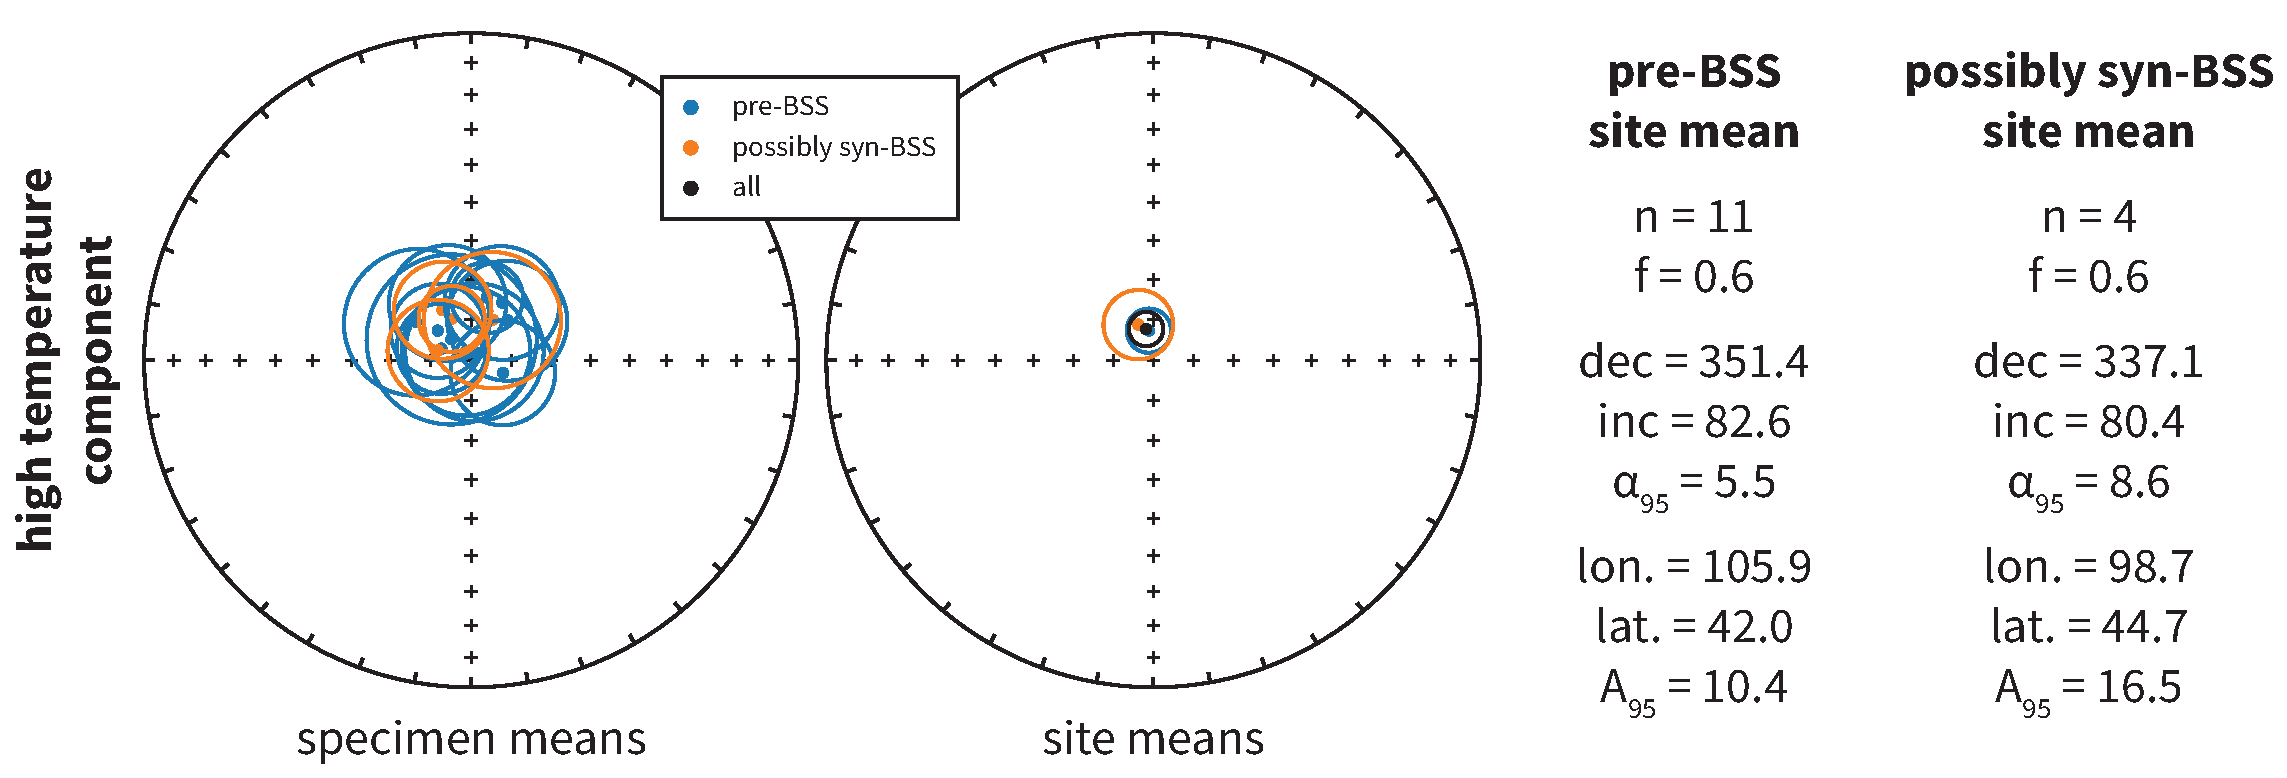
\includegraphics[width=\textwidth]{figures/Xiajiang/lower-upper-comparison.pdf}
    \caption[Comparison of the high temperature component from sites that are pre-Bitter Springs Stage and sites that could be syn-Bitter Springs Stage.]{Comparison of the high temperature component from sites that are unambiguously constrained by the geochronology to be pre-Bitter Springs Stage and sites that could be syn-Bitter Springs Stage (Fig. \ref{fig:stratigraphic-sections}). The angular difference between the two site mean directions is 3.0\degrees.}
    \label{fig:lower-upper-comparison}
\end{figure}

We compare the high temperature components obtained from the 11 sites that are unambiguously pre-Bitter Springs Stage, with the high temperature components obtained from the four sites that could be syn-Bitter Springs Stage. After converting all sites into a single polarity and applying a tilt and inclination correction, the two site mean directions have an angular difference of 3.0\degrees, and a common mean test cannot reject the null hypothesis at the 95\% confidence level that the specimen mean directions were drawn from distributions that share a common mean direction (in the Watson V test, $V$ = 0.8 and $V_{crit}$ = 6.9; Fig. \ref{fig:lower-upper-comparison}). This angular difference is much less than would be expected for Bitter Springs Stage TPW, indicating that the Nanhua Basin was in a similar position throughout Xiajiang Group deposition and that the sites can be grouped into a single paleomagnetic pole. However, ambiguity surrounding the age of the 4 sites that could be syn-Bitter Springs Stage hinders the ability to draw firm conclusions regarding TPW using the Xiajiang Group data alone. To gain more robust insight, we can assess the Xiajiang Group data in the context of the other Tonian South China poles.

The new 813$\pm$3~Ma Xiajiang Group pole and the new 804.9$\pm$0.4~Ma date on the Madiyi Formation pole provide paleomagnetic constraints on the position of South China before and during the Bitter Springs Stage. Additionally, the 821.6$\pm$0.2~Ma date on the Xiaofeng dikes pole constrains it to be pre-Bitter Springs Stage (although prior interpretations have taken the Xiaofeng dikes pole to represent a syn-Bitter Springs Stage position of South China using its previously assigned age of 802$\pm$10~Ma; \citealp{Maloof2006a, Jing2019a}). The pre-Bitter Springs Stage Xiaofeng dikes pole and the syn-Bitter Springs Stage Madiyi Formation pole share a common mean (Fig. \ref{fig:SChina-APWP}). Interpreting these two poles alone would suggest that South China was in a stable position between ca. 821 and 805~Ma in contrast to the prediction of the TPW hypothesis.

\begin{figure}[h!]
    \centering
    \includegraphics[width=\textwidth]{figures/Xiajiang/TPW-MC.pdf}
    \caption[Results of Monte Carlo analysis of hypothesized ca. 810~Ma rapid true polar wander motion.]{Results of Monte Carlo analysis of hypothesized ca. 810~Ma rapid true polar wander motion. \textbf{A)} Virtual geomagnetic poles (VGPs) for the Xiajiang Group, Madiyi Formation, and Lower and Upper Grusdievbreen Formation paleomagnetic poles randomly sampled from Fisherian distributions ($n=10,000$). South China is shown in its present day location, and Svalbard is rotated such that the 4 poles lie along a great circle. \textbf{B)} Ages of the Xiajiang Group and Madiyi Formation poles randomly sampled from uniform and Gaussian distributions respectively. \textbf{C)} Angular difference between randomly selected VGP pairs in A. \textbf{D)} Plate velocity of South China implied by A and B, and the plate velocity of Svalbard implied by A and assuming that the Upper Grusdievbreen Formation pole is 1--10~m.y. younger than the Lower Grusdievbreen Formation pole. The dashed vertical line is the $\sim$20~cm/yr plate velocity limit suggested by \citet{Conrad2001a} and \citet{Zahirovic2015a}.}
    \label{fig:TPW-MC}
\end{figure}

\begin{figure}[!htbp]
    \centering
    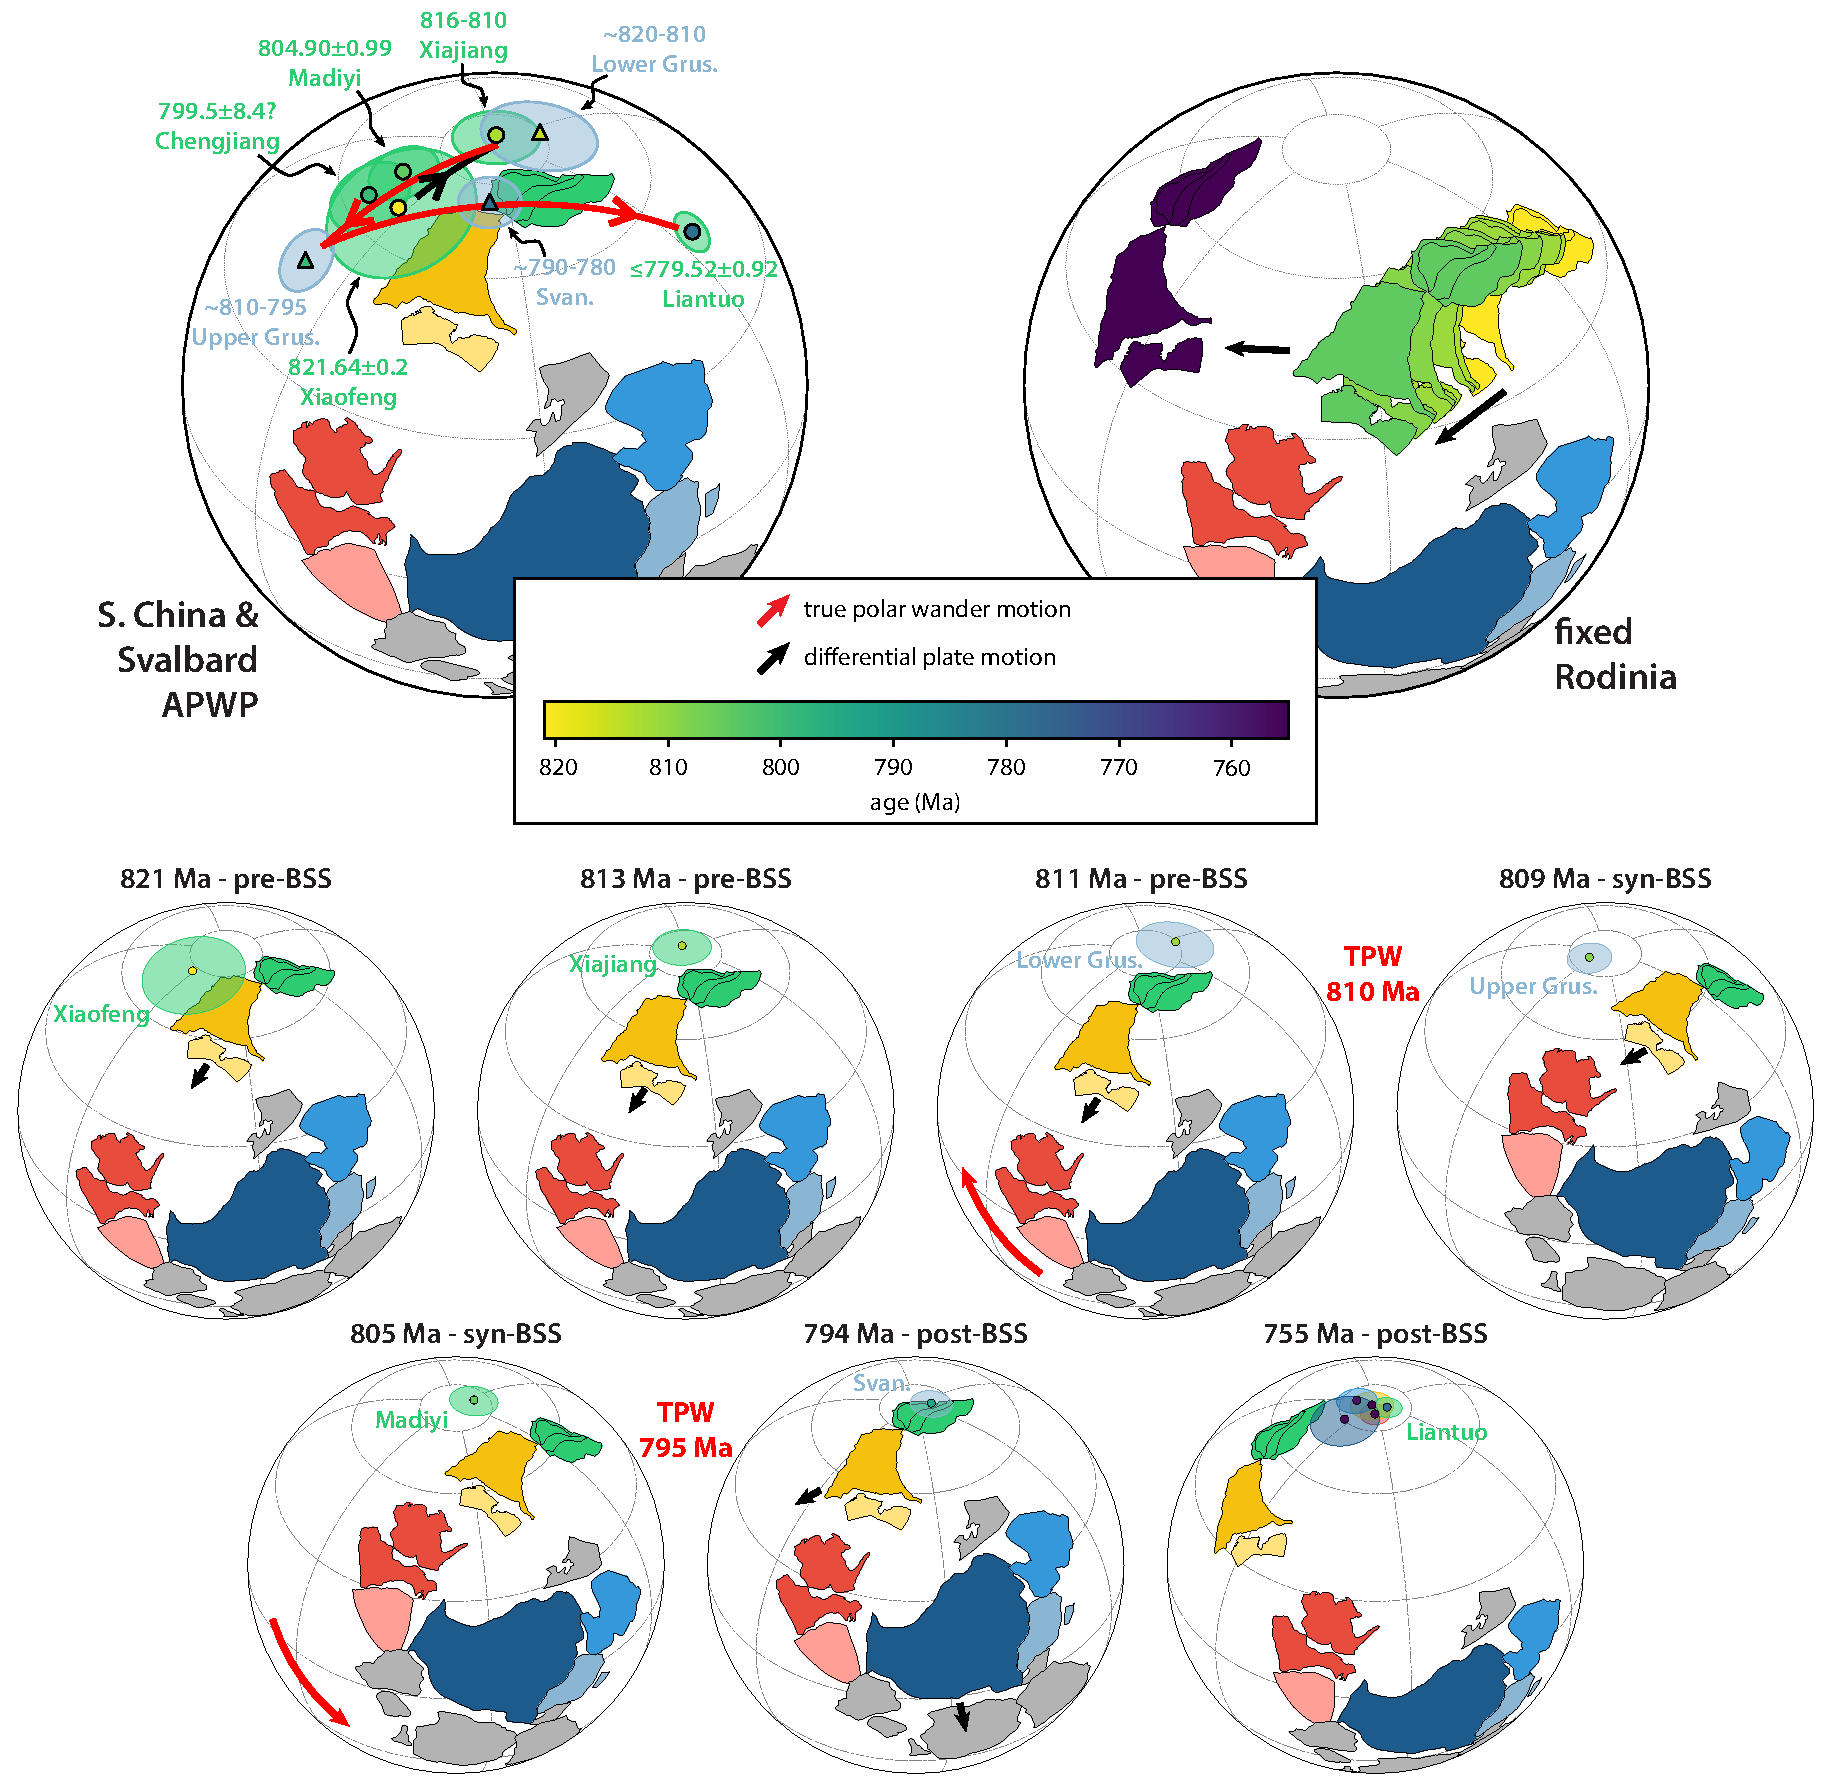
\includegraphics[width=\textwidth]{figures/Xiajiang/BSS-APWP.pdf}
    \caption[Continuous paleogeographic model if Tonian paleomagnetic poles from South China are interpreted as recording differential plate motion superimposed upon Bitter Springs Stage true polar wander.]{Continuous paleogeographic model if Tonian paleomagnetic poles from South China are interpreted as recording differential plate motion superimposed upon Bitter Springs Stage (BSS) true polar wander (TPW). In the upper left, the tectonic blocks are shown in a ca. 813~Ma reconstruction, and the apparent polar wander paths (APWPs) of South China and Svalbard are aligned along two great circles. In the upper right, Rodinia (Laurentia + associated cratons) is fixed in a ca. 755~Ma reconstruction to show the differential motion of South China-India-Rayner relative to Rodinia. The seven lower reconstructions show pre-, syn-, and post-BSS reconstructions in a celestial reference frame. Note that differential plate motion of South China-India-Rayner continues through ca. 810~Ma rapid TPW defined by the Lower and Upper Grusdievbreen Formation poles of Svalbard. Euler rotations for this paleogeographic model are shown in Table S9.}
    \label{fig:BSS-APWP}
\end{figure}

However, the pre-Bitter Springs Stage Xiajiang Group pole has a distinct position from the syn-Bitter Springs Stage Madiyi Formation pole, with an angular difference of 19\degrees between the means of the poles (Fig. \ref{fig:SChina-APWP}). In order to assess this angular difference in comparison to the poles from Svalbard while accounting for the uncertainty on the pole positions and ages, we take a Monte Carlo approach in which 10,000 random draws are taken from Fisherian distributions for the pole positions and from Gaussian distributions for the pole ages (Figs. \ref{fig:TPW-MC}A and \ref{fig:TPW-MC}B; \citealp{Swanson-Hysell2014b}). Taking this approach, the angular difference between the Xiajiang Group and Madiyi Formation poles is 11--27\degrees at the 95\% confidence level, whereas the angular difference between the Lower and Upper Grusdievbreen Formation poles is much higher at 41--62\degrees at the 95\% confidence level (Fig. \ref{fig:TPW-MC}C). In fact, the probability that a Xiajiang Group--Madiyi Formation pole pair has an equal or larger angular difference than a Lower--Upper Grusdievbreen Formation pole pair is only 8.5$\times$10$^{-5}$\% (calculated using the means and standard deviations of the normal distributions in Fig. \ref{fig:TPW-MC}C). As such, the angular difference between the pre-Bitter Springs and syn-Bitter Springs poles is significantly less than that predicted by the TPW hypothesis based on the data from Svalbard. Therefore, this Monte Carlo analysis suggests that the angular difference between the pole pairs from South China and Svalbard can not be straight-forwardly interpreted to be associated with a single TPW rotation.

The velocity of South China implied by the Xiajiang Group and Madiyi Formation poles is also slower than that implied for Svalbard by the Lower and Upper Grusdievbreen Formation poles, being 14--48~cm/yr rather than 60--284~cm/yr at the 95\% confidence level, if the Upper Grusdievbreen Formation pole is taken to be 1 to 10~m.y. younger than the Lower Grusdievbreen Formation pole (\citealp{Maloof2006a}; Fig. \ref{fig:TPW-MC}D). In contrast to the very rapid rates implied by the Svalbard poles, the rate for South China's motion is at the upper end of the range of velocities suggested by plate kinematic reconstructions (Fig. \ref{fig:TPW-MC}D; \citealp{Meert1993a, Zahirovic2015a}).

However, the smaller angular difference between the Xiajiang Group and Madiyi Formation poles relative to the Lower and Upper Grusdievbreen Formation poles could be reconciled with the TPW hypothesis if differential plate motion between South China and Svalbard is superimposed on TPW motion between ca. 813 and 805~Ma \citep{Evans2003a}. For example, if rapid TPW occurred ca. 810~Ma, the Xiajiang Group and Madiyi Formation poles should lie along the great circle between the Lower and Upper Grusdievbreen Formation poles, implying a unique reconstruction for South China relative to Svalbard (Fig. \ref{fig:BSS-APWP}). This configuration also aligns the great circle between the syn-Bitter Springs Stage Upper Grusdievbreen Formation and post-Bitter Springs Stage Svanbergfjellet Formation Svalbard poles with that of the syn-Bitter Springs Stage Madiyi Formation and post-Bitter Springs Stage Liantuo Formation South China poles (Fig. \ref{fig:BSS-APWP}). In the TPW hypothesis, this second great circle would represent the second rapid TPW event ca. 795~Ma. However, South China could have continued to move via differential plate tectonics along the trajectory implied by the difference between the ca. 821~Ma Xiaofeng dikes and the ca. 813~Ma Xiajiang Formation poles through ca. 810~Ma TPW rotation (Fig. \ref{fig:BSS-APWP}). In such a scenario, the differential plate tectonic motion of South China is approximately opposite the trajectory of the hypothesized TPW rotation (Fig. \ref{fig:BSS-APWP}), which would be observed in the paleomagnetic record as a smaller angular difference between pre- to syn-Bitter Springs Stage paleomagnetic poles from South China than what would be predicted for TPW alone. Put another way, differential plate tectonic motion could have driven South China in the opposite direction of TPW motion, causing South China to move a smaller distance in a celestial reference frame relative to other tectonic blocks that were not experiencing such differential plate tectonic motion between ca. 813 and 805~Ma, such as Svalbard.

Importantly, if rapid TPW did occur ca. 810~Ma, and differential plate motion between South China and Svalbard ca. 813--805~Ma is superimposed upon that TPW motion to explain the smaller angular difference between the Xiajiang Group and Madiyi Formation poles relative to the Lower and Upper Grusdievbreen Formation poles, then it is required that South China was separate from Rodinia (i.e. the Separate model in Figure \ref{fig:Rodinia-models}). It is well established that Svalbard was connected to Laurentia via Greenland until Silurian-Devonian translation along Greenland's margin and subsequent rifting away from Greenland in the Eocene \citep{Torsvik2016a}. Therefore, if South China was moving differentially relative to Svalbard ca. 813--805~Ma, South China must have been moving differentially relative to Rodinia, and therefore must have been separate from Rodinia. Furthermore, the alignment of paleomagnetic poles from South China and Svalbard along great circles places South China at high latitudes, with the long southeastern margin of the Cathaysia block facing Svalbard (Fig. \ref{fig:BSS-APWP}). However, ca. 755~Ma paleomagnetic poles require that a Periphery model has South China-India-Rayner connected to Rodinia in a different orientation via northwestern Australia (Fig. \ref{fig:Rodinia-models}).

Regardless of whether the ca. 821~Ma to ca. 805~Ma poles are interpreted as recording a reduced magnitude of TPW counteracted by plate tectonic motion or indicating a relatively stable position of South China (as in Figure \ref{fig:SChina-APWP}F), South China is peripheral or disconnected from Rodinia.

\section{Conclusions}

The geochronologic and paleomagnetic data developed from the Xiajiang Group constrain the amalgamation of the Yangtze and Cathaysia blocks of South China to have occurred between ca. 830~Ma and 815.73$\pm$0.18~Ma at high latitudes. A consistent high latitude position is implied by poles from ca. 821~Ma to 805~Ma with a continued high latitude position ca. 780~Ma following South China transiting over the pole. These paleolatitudes, as well as convergent orogenesis between the Yangtze and Cathaysia blocks and continued arc activity along the northwest margin of the South China craton during the Tonian and into the Cryogenian, cannot be reconciled with the Missing Link model that places South China in the core of a stable Rodinia continent. The angular difference in pole position between the ca. 813~Ma (pre-Bitter Springs Stage) Xiajiang Group pole and ca. 805~Ma (syn-Bitter Springs Stage) Madiyi Formation pole is significantly less than that predicted for the Bitter Springs Stage TPW hypothesis. The poles could be interpreted to indicate a relatively stable high latitude position for South China inconsistent with TPW. However, it is possible to interpret the poles as TPW rotation counteracted by plate tectonic motion. In this scenario, South China must be considered to be distinct from Rodinia. Whether or not the paleomagnetic poles are interpreted as recording TPW, they constrain South China to either have been connected to Rodinia along its periphery, or disconnected from the (super)continent entirely.

\section{Acknowledgements}

Research was supported by National Science Foundation Grants EAR-1547434 and EAR-1547537. Maoyan Zhu supported research logistics in the field. Oliver Abbitt prepared specimens for paleomagnetic analyses.
